\documentclass[10pt,aspectratio=169]{beamer}

% Font encoding and font packages
\usepackage[T1]{fontenc}
\usepackage{lmodern}

% Theme and styling
\usetheme{Madrid}
\usecolortheme{default}
\setbeamertemplate{navigation symbols}{}
\setbeamertemplate{footline}[frame number]

% Increase title slide font sizes
\setbeamerfont{title}{size=\Huge,series=\bfseries}
\setbeamerfont{author}{size=\Large}
\setbeamerfont{institute}{size=\large}
\setbeamerfont{date}{size=\large}

% Packages
\usepackage{amsmath}
\usepackage{amssymb}
\usepackage{pifont}
\usepackage{xcolor}
\usepackage{tikz}
\usepackage{subcaption}
\usepackage{graphicx}
\usepackage{algorithm}
\usepackage{algorithmicx}
\usepackage{algpseudocode}
% \usepackage{enumitem}  % Conflicts with beamer
\usepackage{mathtools}
\usepackage{bm}

\definecolor{mygreen}{rgb}{0,0.6,0}
\definecolor{myred}{rgb}{0.8,0,0}
\newcommand{\greenoplus}{\textcolor{mygreen}{\ding{51}}}
\newcommand{\redominus}{\textcolor{myred}{\ding{55}}}

% Custom commands
\newcommand{\R}{\mathbb{R}}
\DeclareMathOperator{\atan}{atan2}

% Title information
\title{Scene Representation Paradigms for \\ Multimodal Trajectory Prediction}
\author{Lukas Röß \and Jan Duscherer}
\institute{%
  Seminar: \textbf{Video Analysis and Object Tracking}\\[0.5ex]
  Department of Computer Science and Mathematics\\[1ex]
  Lecturer: Prof.\ Dr.\ Claudius Schnörr
}
\date{\today}
\titlegraphic{%
  \vspace{1em}%
  \hfill
\includegraphics[height=1.5cm]{docs/latex/figures/hm-logo.pdf}%
}

\begin{document}

% Title slide
\begin{frame}[plain]
  \titlepage
\end{frame}

% Outline slide
\begin{frame}{Outline}
\tableofcontents
\end{frame}

\section{Scene Representation Paradigms}

\begin{frame}[plain]
  \begin{center}
    \vfill
    {\Huge \textbf{Scene Representation Paradigms}}
    \vfill
    {\Large for Multimodal Trajectory Prediction}
    \vfill
  \end{center}
\end{frame}

\begin{frame}{Why Scene Representations Matter}
\begin{block}{Core Challenge}
How do we translate perception outputs into tensors that neural modules can effectively exploit for trajectory prediction?
\end{block}

\vspace{0.5cm}

\begin{columns}[T]
\column{0.6\textwidth}
\textbf{Desirable Properties:}
\begin{enumerate}
    \item High geometric fidelity
    \item Invariance to global transformations $SE(2) \rtimes \mathbb{R} \times S_n$\footnote{Roto-translation + time translation + permutation}
    \item Information density
    \item Efficient spatio-temporal modeling
    \item Computational re-use across frames
\end{enumerate}

\column{0.35\textwidth}
\begin{alertblock}{Impact}
The choice of scene representation fundamentally affects the predictor's capacity to capture essential relationships and produce accurate motion forecasts.
\end{alertblock}
\end{columns}
\end{frame}

\begin{frame}{Two Main Paradigms}
\begin{figure}
\centering
\begin{subfigure}[t]{0.45\textwidth}
    \centering
    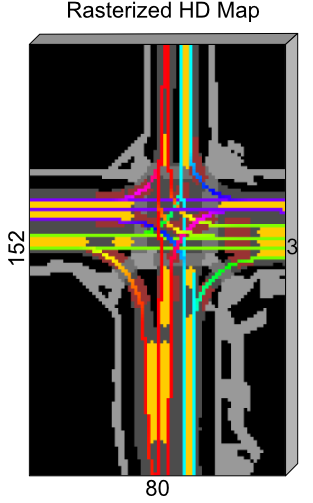
\includegraphics[width=0.6\columnwidth,height=0.5\textheight,keepaspectratio]{docs/latex/figures/caspnet-bev-repr.png}
    \caption{Rasterized BEV encoding~\cite{caspnetSchäfer2022}}
    \label{fig:rasterized}
\end{subfigure}
\hfill
\begin{subfigure}[t]{0.5\textwidth}
    \centering
    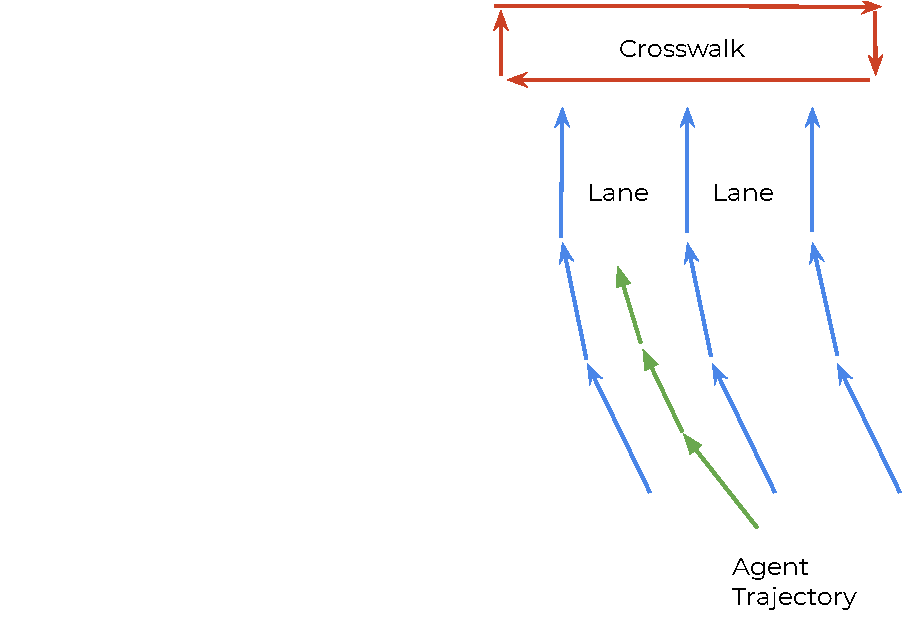
\includegraphics[width=0.6\columnwidth,height=0.5\textheight,keepaspectratio]{docs/latex/figures/vectornet-2020-vector-repr.pdf}
    \caption{Vectorized polyline preservation~\cite{gao2020vectornet}}
    \label{fig:vectorized}
\end{subfigure}
\end{figure}

\vspace{0.5em}
\begin{itemize}
    \item \textbf{Rasterized}: Stack trajectories and HD maps into BEV images
    \item \textbf{Vectorized}: Preserve geometric polylines and relationships
\end{itemize}
\end{frame}

\subsection{Rasterized Approaches}

\begin{frame}{Raster Grid Representations}
\begin{columns}[T]
\column{0.6\textwidth}
\textbf{Key Components:}
\begin{itemize}
    \item BEV stack of past agent trajectories: $\mathbf{I}_d \in \mathbb{R}^{T_p \times H \times W \times F_d}$
    \item Static HD-map raster: $\mathbf{I}_s \in \mathbb{R}^{H \times W \times F_s}$
    \item Leverage convolutional backbones
    \item Runtime independent of number of agents
\end{itemize}

\textbf{Examples:} CASPNet~\cite{caspnetSchäfer2022}, CASPFormer~\cite{caspformerYadav2024}, MultiPath~\cite{chai2019multipath}

\column{0.35\textwidth}
\begin{block}{Advantages}
\begin{itemize}
    \item Mature CNN paradigms
    \item Runtime independent of number of agents
\end{itemize}
\end{block}

\begin{alertblock}{Limitations~\cite{gao2020vectornet}}
\begin{itemize}
    \item Limited geometric fidelity
    \item Redundant pixel information
    \item Doesn't respect identities
    \item Shared coordinate system only
    \item Invariance only for center agent
\end{itemize}
\end{alertblock}
\end{columns}
\end{frame}

\subsection{Vectorized Approaches}

\begin{frame}{Vector Representations}
\textbf{Core Principle:} Encode agents and lanes as vectorized geometric primitives (Cartesian or polar coordinates)

\vspace{0.3cm}

\begin{columns}[T]
\column{0.48\textwidth}
\textbf{Lane Representations:}
\begin{itemize}
    \item \textbf{Point-based}: $L_p^i = [P_1^i, P_2^i, \ldots, P_K^i]$~\cite{VectorNet2020, zhou2022hivt}
    \item \textbf{Segment-based}: $L_v^i = [V_1^i, V_2^i, \ldots, V_{K-1}^i]$ where $V_{k}^i = [P_k^i, P_{k+1}^i]$~\cite{liang2020learning,zhou2022hivt}
\end{itemize}

\column{0.48\textwidth}
\textbf{Agent Trajectories:}
\begin{itemize}
    \item \textbf{Trajectory points}: $\mathcal{T}_{in}^a = [P_1^a, P_2^a, \ldots, P_T^a]$
    \item \textbf{Motion vectors}: $M_t^a = [P_{2}^a - P_{1}^a, \ldots, P_{T}^a - P_{T-1}^a]$~\cite{lmformerYadav2025}
\end{itemize}
\end{columns}

\vspace{0.3cm}

\begin{block}{Key Benefits~\cite{VectorNet2020, lmformerYadav2025}}
\begin{itemize}
    \item Higher geometric fidelity
    \item Explicit modeling of spatio-temporal relationships
    \item Enables graph/transformer architectures
    \item More compact representation
\end{itemize}
\end{block}
\end{frame}

\section{Query-Centric Paradigm}

\begin{frame}[plain]
  \begin{center}
    \vfill
    {\Huge \textbf{Query-Centric Paradigm}}
    \vfill
    {\Large Breaking Free from Agent-Centric Limitations\\\vspace{0.5em}\emph{Local Space-Time Manifolds} for Symmetry and Efficiency}
    \vfill
  \end{center}
\end{frame}

\begin{frame}{Limitations of Agent-Centric Approaches}
\begin{columns}[T]
\column{0.65\textwidth}
\textbf{Agent-Centric Issues~\cite{qcnetZhou2023}:}
\begin{itemize}
    \item Single global frame centered on ego vehicle
    \item Roto-translation invariance only for center agent
    \item No permutation invariance (center agent privileged)
    \item Computationally infeasible for attention-based models
    \item Must re-encode entire scene at each timestep
\end{itemize}

\textbf{Factorized Attention Complexity:}
Factorized attention simplifies full attention by computing interactions along only one dimension at a time (e.g., temporal or spatial), while keeping other dimensions fixed.

\begin{align}
\text{Temporal:} &\quad \mathcal{O}(N_{A}T^{2}) \\
\text{Agent}\leftrightarrow\text{Map Fusion:} &\quad \mathcal{O}(N_{A}T N_{M}) \\
\text{Agent}\leftrightarrow\text{Agent Fusion:} &\quad \mathcal{O}(N_{A}^{2}T)
\end{align}

\column{0.3\textwidth}
\begin{alertblock}{Problem}
Cubic complexity in dense traffic scenarios leads to significant computational overhead.
\end{alertblock}
\end{columns}
\end{frame}

\begin{frame}{Query-Centric Solution}
\begin{figure}[ht]
\centering
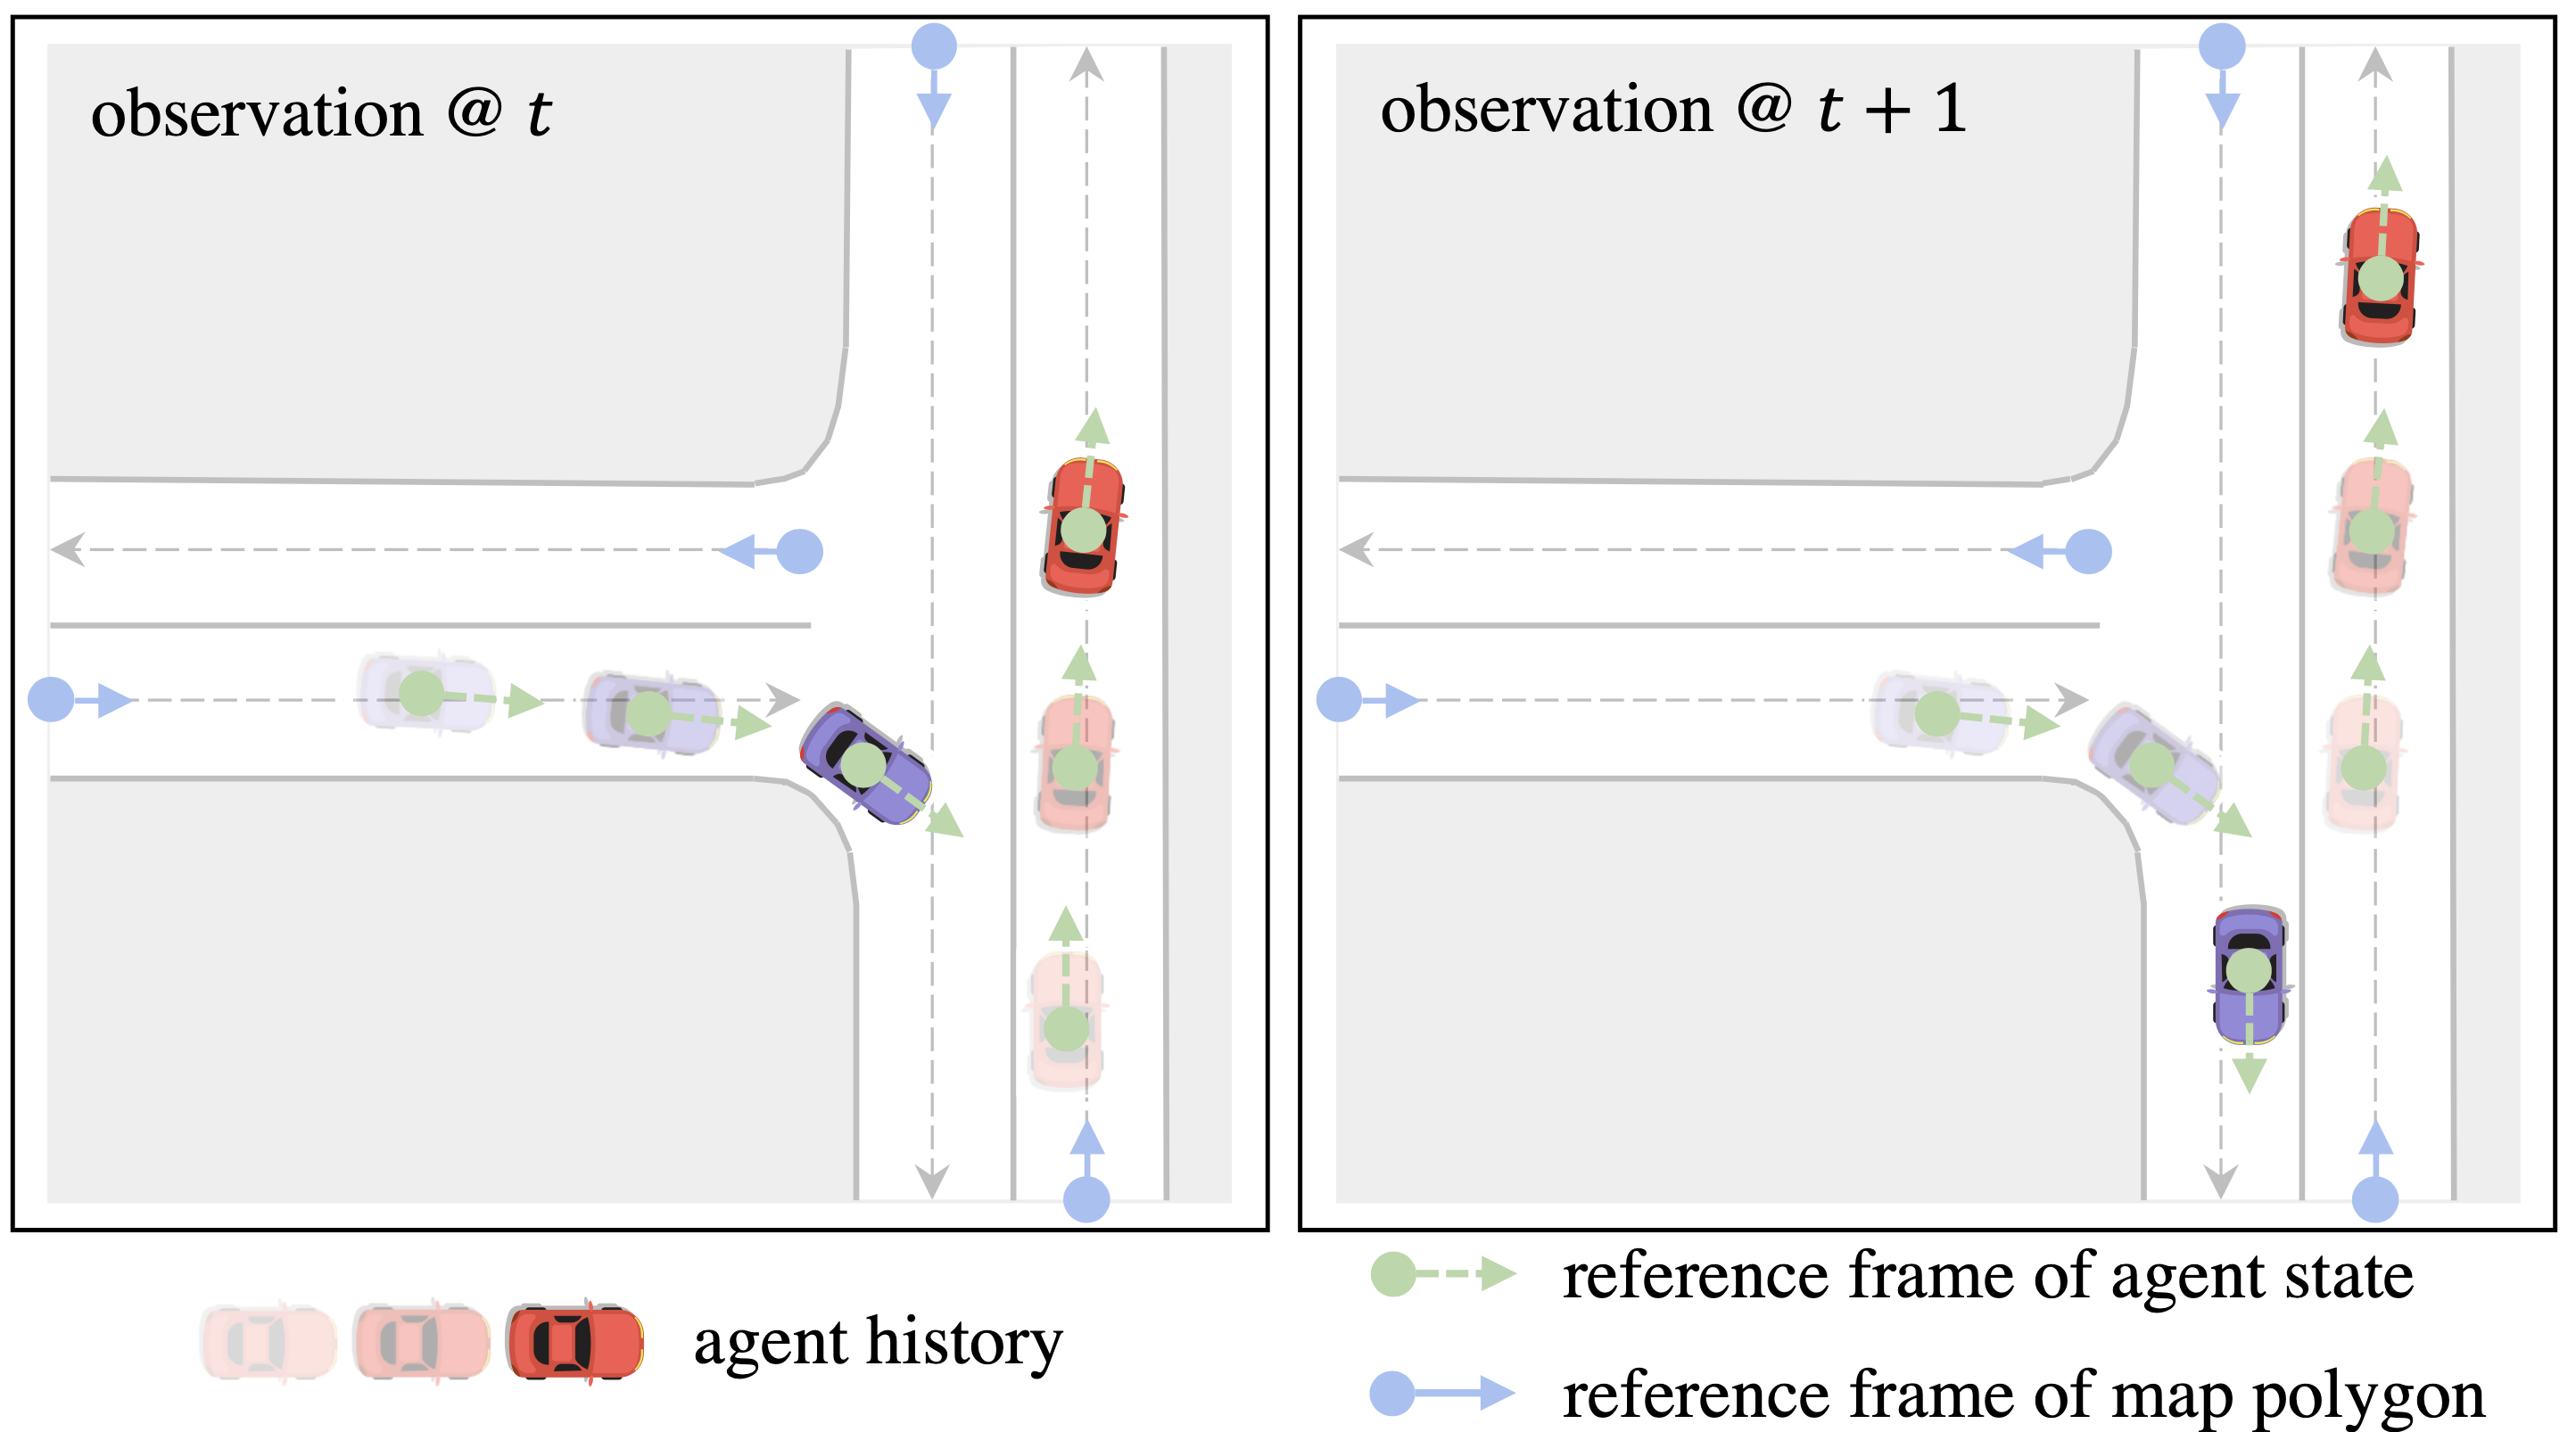
\includegraphics[width=0.6\textwidth, height=0.4\textheight, keepaspectratio]{docs/latex/figures/qc_reference_frame.png}
\caption{Each scene entity lives in its own local coordinate system~\cite{qcnetZhou2023}}
\end{figure}

\textbf{Key Insight:} Establish a \emph{fiber} (local space-time coordinate system) for each scene element~\cite{qcnetZhou2023}

\begin{block}{Computational Benefits~\cite{qcnetZhou2023}}
\begin{center}
\footnotesize
$\underbrace{\mathcal{O}(N_{A}T^2)+\mathcal{O}(N_{A}TN_M)+\mathcal{O}(N_{A}^2T)}_{\text{agent-centric (A2T, A2M, A2A)}}
\longrightarrow
\underbrace{\mathcal{O}(N_{A}T)+\mathcal{O}(N_{A}N_M)+\mathcal{O}(N_{A}^2)}_{\text{query-centric (A2T, A2M, A2A)}}$
\end{center}
\end{block}
\begin{center}
Cubic \( \rightarrow \) quadratic complexity for attention operations
\end{center}
\end{frame}

\subsection{Local Frame Construction}

\begin{frame}{Local Frame Construction}
\textbf{Agent States:} For the $i$-th agent at timestep $t$, local frame anchored at $\mathbf{p}_i^t = (p_{i,x}^t, p_{i,y}^t)$ with $x$-axis aligned to heading $\theta_i^t$:

\begin{equation}
\mathbf{x}^{(i,t)}_{\text{local}} = \mathbf{T}_{i,t}^{-1} \mathbf{x}_{\text{global}}^{(i,t)}, \quad
\mathbf{T}_{i,t} = \begin{bmatrix}
\cos\theta_i^t & -\sin\theta_i^t & p_{i,x}^t \\
\sin\theta_i^t & \cos\theta_i^t & p_{i,y}^t \\
0 & 0 & 1
\end{bmatrix} \in \mathrm{SE}(2)
\end{equation}

\vspace{0.3cm}

\textbf{Map Elements:} Each segment's start vertex acts as origin, first segment direction defines $x$-axis

\begin{block}{Result~\cite{qcnetZhou2023}}
$N_{A} \times T + N_M$ distinct fibers over observation window, each with standardized local representation
\end{block}
\end{frame}

\begin{frame}{Fiber Bundle Visualization}
\begin{block}{Visualizing the Decomposition}
The global scene (manifold $\mathcal{M}$) is decomposed into a \emph{fiber-bundle}, each with it's own local coordinate system ($f_1, f_2, \ldots, f_{N_AT+N_M})$. Spatial and kinematic features are represented locally as vectors $(r, \theta)$, and \emph{connections} between fibers are captured by \emph{relative descriptors} ($\mathbf{r}_{j\to i}$).
\end{block}
\begin{figure}[ht]
\centering
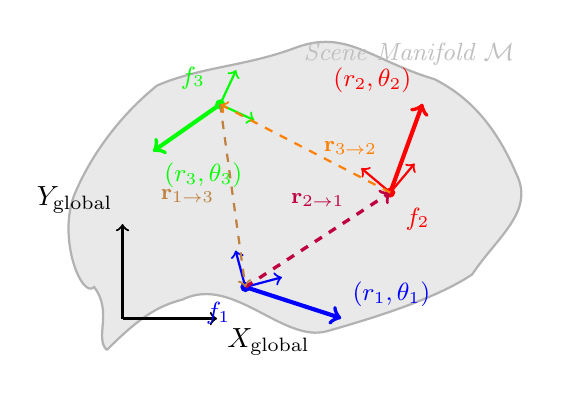
\begin{tikzpicture}[scale=0.8]
  % Complex 2D manifold
  \coordinate (origin) at (0,0);
  \coordinate (p1) at (1.2,0.8);
  \coordinate (p2) at (3.5,0.3);
  \coordinate (p3) at (5.8,1.2);
  \coordinate (p4) at (6.5,2.8);
  \coordinate (p5) at (5.2,4.3);
  \coordinate (p6) at (3.0,4.8);
  \coordinate (p7) at (0.8,4.2);
  \coordinate (p8) at (-0.5,2.5);
  \coordinate (p9) at (-0.2,1.0);

  % Manifold surface
  \fill [gray!25, opacity=0.7]
        (origin) ..
        controls (0.5,0.5) and (0.8,0.7) ..
        (p1) ..
        controls (2.0,1.2) and (2.8,0.1) ..
        (p2) ..
        controls (4.2,0.5) and (5.2,0.8) ..
        (p3) ..
        controls (6.2,1.8) and (6.8,2.2) ..
        (p4) ..
        controls (6.2,3.5) and (5.8,4.0) ..
        (p5) ..
        controls (4.2,4.6) and (3.8,5.1) ..
        (p6) ..
        controls (2.2,4.5) and (1.5,4.5) ..
        (p7) ..
        controls (0.3,3.8) and (-0.2,3.2) ..
        (p8) ..
        controls (-0.8,1.8) and (-0.4,0.8) ..
        (p9) ..
        controls (0.1,0.6) and (-0.2,0.2) ..
        (origin) -- cycle;

  % Manifold boundary
  \draw [gray!60, thick]
        (origin) ..
        controls (0.5,0.5) and (0.8,0.7) ..
        (p1) ..
        controls (2.0,1.2) and (2.8,0.1) ..
        (p2) ..
        controls (4.2,0.5) and (5.2,0.8) ..
        (p3) ..
        controls (6.2,1.8) and (6.8,2.2) ..
        (p4) ..
        controls (6.2,3.5) and (5.8,4.0) ..
        (p5) ..
        controls (4.2,4.6) and (3.8,5.1) ..
        (p6) ..
        controls (2.2,4.5) and (1.5,4.5) ..
        (p7) ..
        controls (0.3,3.8) and (-0.2,3.2) ..
        (p8) ..
        controls (-0.8,1.8) and (-0.4,0.8) ..
        (p9) ..
        controls (0.1,0.6) and (-0.2,0.2) ..
        (origin);

  \node[gray!50, font=\small\itshape] at (4.8,4.7) {Scene Manifold $\mathcal{M}$};

  % Global axes
  \draw[thick,->] (0.25,0.5) -- (1.75,0.5) node[anchor=north west]{$X_{\text{global}}$};
  \draw[thick,->] (0.25,0.5) -- (0.25,2) node[anchor=south east]{$Y_{\text{global}}$};

  % Fiber positions
  \coordinate (e1) at (2.2,1.0);
  \coordinate (e2) at (4.5,2.5);
  \coordinate (e3) at (1.8,3.9);

  % Fiber origins
  \draw[blue,fill=blue]   (e1) circle(2pt) node[below left=2pt] {\small$f_1$};
  \draw[red,fill=red]     (e2) circle(2pt) node[below right=2pt] {\small$f_2$};
  \draw[green,fill=green] (e3) circle(2pt) node[above left=2pt] {\small$f_3$};

  % Local reference frames
  \draw[blue,thick,->]   (e1) -- ++(15:0.6)  node[anchor=south west] {};
  \draw[blue,thick,->]   (e1) -- ++(105:0.6) node[anchor=south east] {};

  \draw[red,thick,->]    (e2) -- ++(50:0.6)  node[anchor=south west] {};
  \draw[red,thick,->]    (e2) -- ++(140:0.6) node[anchor=south east] {};

  \draw[green,thick,->]  (e3) -- ++(-25:0.6) node[anchor=north west] {};
  \draw[green,thick,->]  (e3) -- ++(65:0.6)  node[anchor=south west] {};

  % Motion vectors in local coordinates
  \draw[blue,->,line width=1.5pt]   (e1) -- ++( -18:1.6) node[anchor=south west] {\small$(r_1,\theta_1)$};
  \draw[red,->,line width=1.5pt]    (e2) -- ++(70:1.5) node[anchor=south east] {\small$(r_2,\theta_2)$};
  \draw[green,->,line width=1.5pt]  (e3) -- ++(-145:1.3) node[anchor=north west] {\small$(r_3,\theta_3)$};

  % Relative descriptors
  \draw[purple,dashed,->,very thick] (e1) -- (e2)
    node[midway,above=8pt,align=center] {\footnotesize$\mathbf{r}_{2\to 1}$};
  \draw[orange,dashed,->,thick] (e2) -- (e3)
    node[midway,right=3pt] {\footnotesize$\mathbf{r}_{3\to 2}$};
  \draw[brown,dashed,->,thick]  (e3) -- (e1)
    node[midway,left=3pt] {\footnotesize$\mathbf{r}_{1\to 3}$};
\end{tikzpicture}
\caption{Query-centric representation as fiber bundle with local coordinates and relative descriptors~\cite{qcnetZhou2023}}
\end{figure}
\end{frame}

\subsection{Relative Descriptors}

\begin{frame}{Relative Descriptors and Embeddings}
For any pair of scene elements with tuples $(\mathbf{p}_i^t, \theta_i^t, t)$ and $(\mathbf{p}_j^s, \theta_j^s, s)$~\cite{qcnetZhou2023}:

\begin{equation}
\mathbf{r}_{j\to i}^{s\to t} = \left[
    \|\mathbf{p}_j^s-\mathbf{p}_i^t\|_2,\;
    \atan(p_{j,y}^s-p_{i,y}^t, p_{j,x}^s-p_{i,x}^t)-\theta_i^t,\;
    \theta_j^s-\theta_i^t,\;
    s-t
\right]
\end{equation}

\vspace{0.5cm}

\textbf{4D Descriptor Components:}    \begin{enumerate}
    \item \textbf{Distance:} $\|p_j^s-p_i^t\|_2$ - spatial separation
    \item \textbf{Bearing:} $\atan(\cdot)-\theta_i^t$ - relative direction in local frame
    \item \textbf{Orientation:} $\theta_j^s-\theta_i^t$ - relative heading
    \item \textbf{Time:} $s-t$ - temporal offset
\end{enumerate}

\begin{block}{Key Property~\cite{qcnetZhou2023}}
Invariant under global $SE(2)$ transformations, lifted to high-frequency representation via \emph{Fourier features}
\end{block}
\end{frame}

\subsection{Geometric Perspective}

\begin{frame}{Fundamental Symmetries}
Query-centric paradigm exploits three key symmetries~\cite{qcnetZhou2023}:

\vspace{0.3cm}

\begin{description}
\item[\textbf{Permutation Invariance}]
Agents form unordered sets—no element privileged.\\ For permutation $\sigma \in S_n$: $f_{\boldsymbol{\Psi}}(\sigma \cdot \mathcal{S}) = \rho(\sigma) f_{\boldsymbol{\Psi}}(\mathcal{S})$

\item[\textbf{SE(2) Invariance}]
Rigid transformations leave model output unchanged:
\begin{equation}
f_{\boldsymbol{\Psi}}(g \cdot S) = f_{\boldsymbol{\Psi}}(\mathcal{S}) \quad \forall\; g \in SE(2)
\end{equation}

\item[\textbf{Temporal Translation Invariance}]
Sliding time windows: $f(\mathcal{S}(t+\tau)) = f(\mathcal{S}(t))$ for any $\tau \in \mathbb{R}$
\end{description}

\begin{block}{Geometric Insight}
Global scene manifold factorizes into small, redundant sub-manifolds (fibers)—each representing standardized spatial/kinematic variables connected by simple relations. $ f_{\boldsymbol{\Psi}}$ can learn these simpler representations instead of the complex global manifold.
\end{block}
\end{frame}

\begin{frame}{Fiber Bundle Decomposition}
\begin{columns}[T]
\column{0.6\textwidth}
\textbf{Key Hypothesis~\cite{qcnetZhou2023}:}
\begin{itemize}
    \item Model splits capacity between learning:
    \begin{enumerate}
        \item Relations between fibers
        \item Simple structures within fibers
    \end{enumerate}
    \item Avoids learning non-decomposable global manifold
    \item Pairwise encodings inhabit simpler manifold
\end{itemize}

\textbf{Inductive Bias~\cite{qcnetZhou2023}:}
\begin{itemize}
    \item Respects symmetries
    \item Breaks intractable global manifold into small, repeatable sub-manifolds
    \item More data-efficient and interpretable
\end{itemize}

\column{0.35\textwidth}
\begin{block}{Benefits}
\begin{itemize}
    \item Reduced hypothesis space
    \item Better generalization
    \item Computational efficiency through streaming
    \item Natural multi-agent handling
\end{itemize}
\end{block}

\begin{alertblock}{Trade-off}
Query-centric models trade \textbf{compute} for \textbf{memory} - QCNet requires $\sim 160$ GB VRAM for training~\cite{qcnetZhou2023}
\end{alertblock}
\end{columns}
\end{frame}

\subsection{Comparison and Conclusions}


\begin{frame}{Paradigm Comparison}
\begin{table}[ht]
\centering
\footnotesize
\begin{tabular}{|p{2cm}|p{2.5cm}|p{2.5cm}|p{2.5cm}|}
\hline
\textbf{Aspect} & \textbf{Rasterized} & \textbf{Agent-Centric} & \textbf{Query-Centric} \\
\hline
\textbf{Representation} & BEV image grids & Global ego frame & Local coordinate frames \\
\hline
\textbf{Geometric Fidelity} & Limited by discretization & Higher, vector-based & Highest, preserves relationships \\
\hline
\textbf{Computational Complexity} & $\mathcal{O}(H \times W)$ & $\mathcal{O}(N^2T)$ & $\mathcal{O}(N^2)$ streaming \\
\hline
\textbf{Memory Usage} & Moderate & Moderate & High (caching) \\
\hline
\textbf{Invariances} & Partial SE(2) & Only for ego agent & Full SE(2) $\rtimes \mathbb{R} \times S_n$ \\
\hline
\textbf{Multi-agent} & Challenging & Limited symmetry & Natural, symmetric \\
\hline
\textbf{Streaming} & Re-encode scene & Must re-encode & Efficient caching \\
\hline
\textbf{Architecture} & CNN enc. & Transformer/Graph & Transformer/Graph \\
\hline
\end{tabular}
\end{table}

\begin{block}{Key Takeaway}
Query-centric paradigm offers superior theoretical properties and streaming efficiency at the cost of increased memory requirements
\end{block}
\end{frame}

% \begin{frame}{Summary}
% \begin{columns}[T]
% \column{0.5\textwidth}
% \textbf{Key Contributions:}
% \begin{itemize}
%     \item Fundamental symmetries in trajectory prediction
%     \item Fiber bundle geometric perspective
%     \item Computational efficiency through streaming
%     \item Natural multi-agent capabilities
% \end{itemize}

% \textbf{Applications:}
% \begin{itemize}
%     \item QCNet, QCNeXt
%     \item LMFormer
%     \item Modern trajectory prediction models
% \end{itemize}

% \column{0.45\textwidth}
% \begin{block}{Future Directions}
% \begin{itemize}
%     \item Memory optimization techniques
%     \item Sparse attention mechanisms
%     \item Hybrid approaches
%     \item Real-time deployment
% \end{itemize}
% \end{block}

% \begin{alertblock}{Impact}
% Query-centric paradigm represents a fundamental shift towards more principled, efficient, and scalable trajectory prediction
% \end{alertblock}
% \end{columns}
% \end{frame}
% conclusion: MTR effectively disentangles multimodality by using static queries for high-level intentions and dynamic queries for detailed path refinement.


\section{Review of Selected Architectures}

\begin{frame}[plain]
  \begin{center}
    \vfill
    {\Huge \textbf{Review of Selected}}
    \vfill
    {\Huge \textbf{Architectures}}
    \vfill
    {\Large MTR \& LMFormer}
    \vfill
  \end{center}
\end{frame}


%==============================================================================
% MTR Section
%==============================================================================

\subsection{Motion TRansformer (MTR)}

\begin{frame}{Motion TRansformer (MTR): Overview}
    \begin{block}{Core Principle}
        MTR models motion prediction as a two-stage process:
        \begin{enumerate}
            \item \textbf{Global Intention Localization:} Propose a diverse set of high-level goals.
            \item \textbf{Local Movement Refinement:} Generate precise paths to achieve these goals.
        \end{enumerate}
    \end{block}
    \begin{figure}
        \centering
        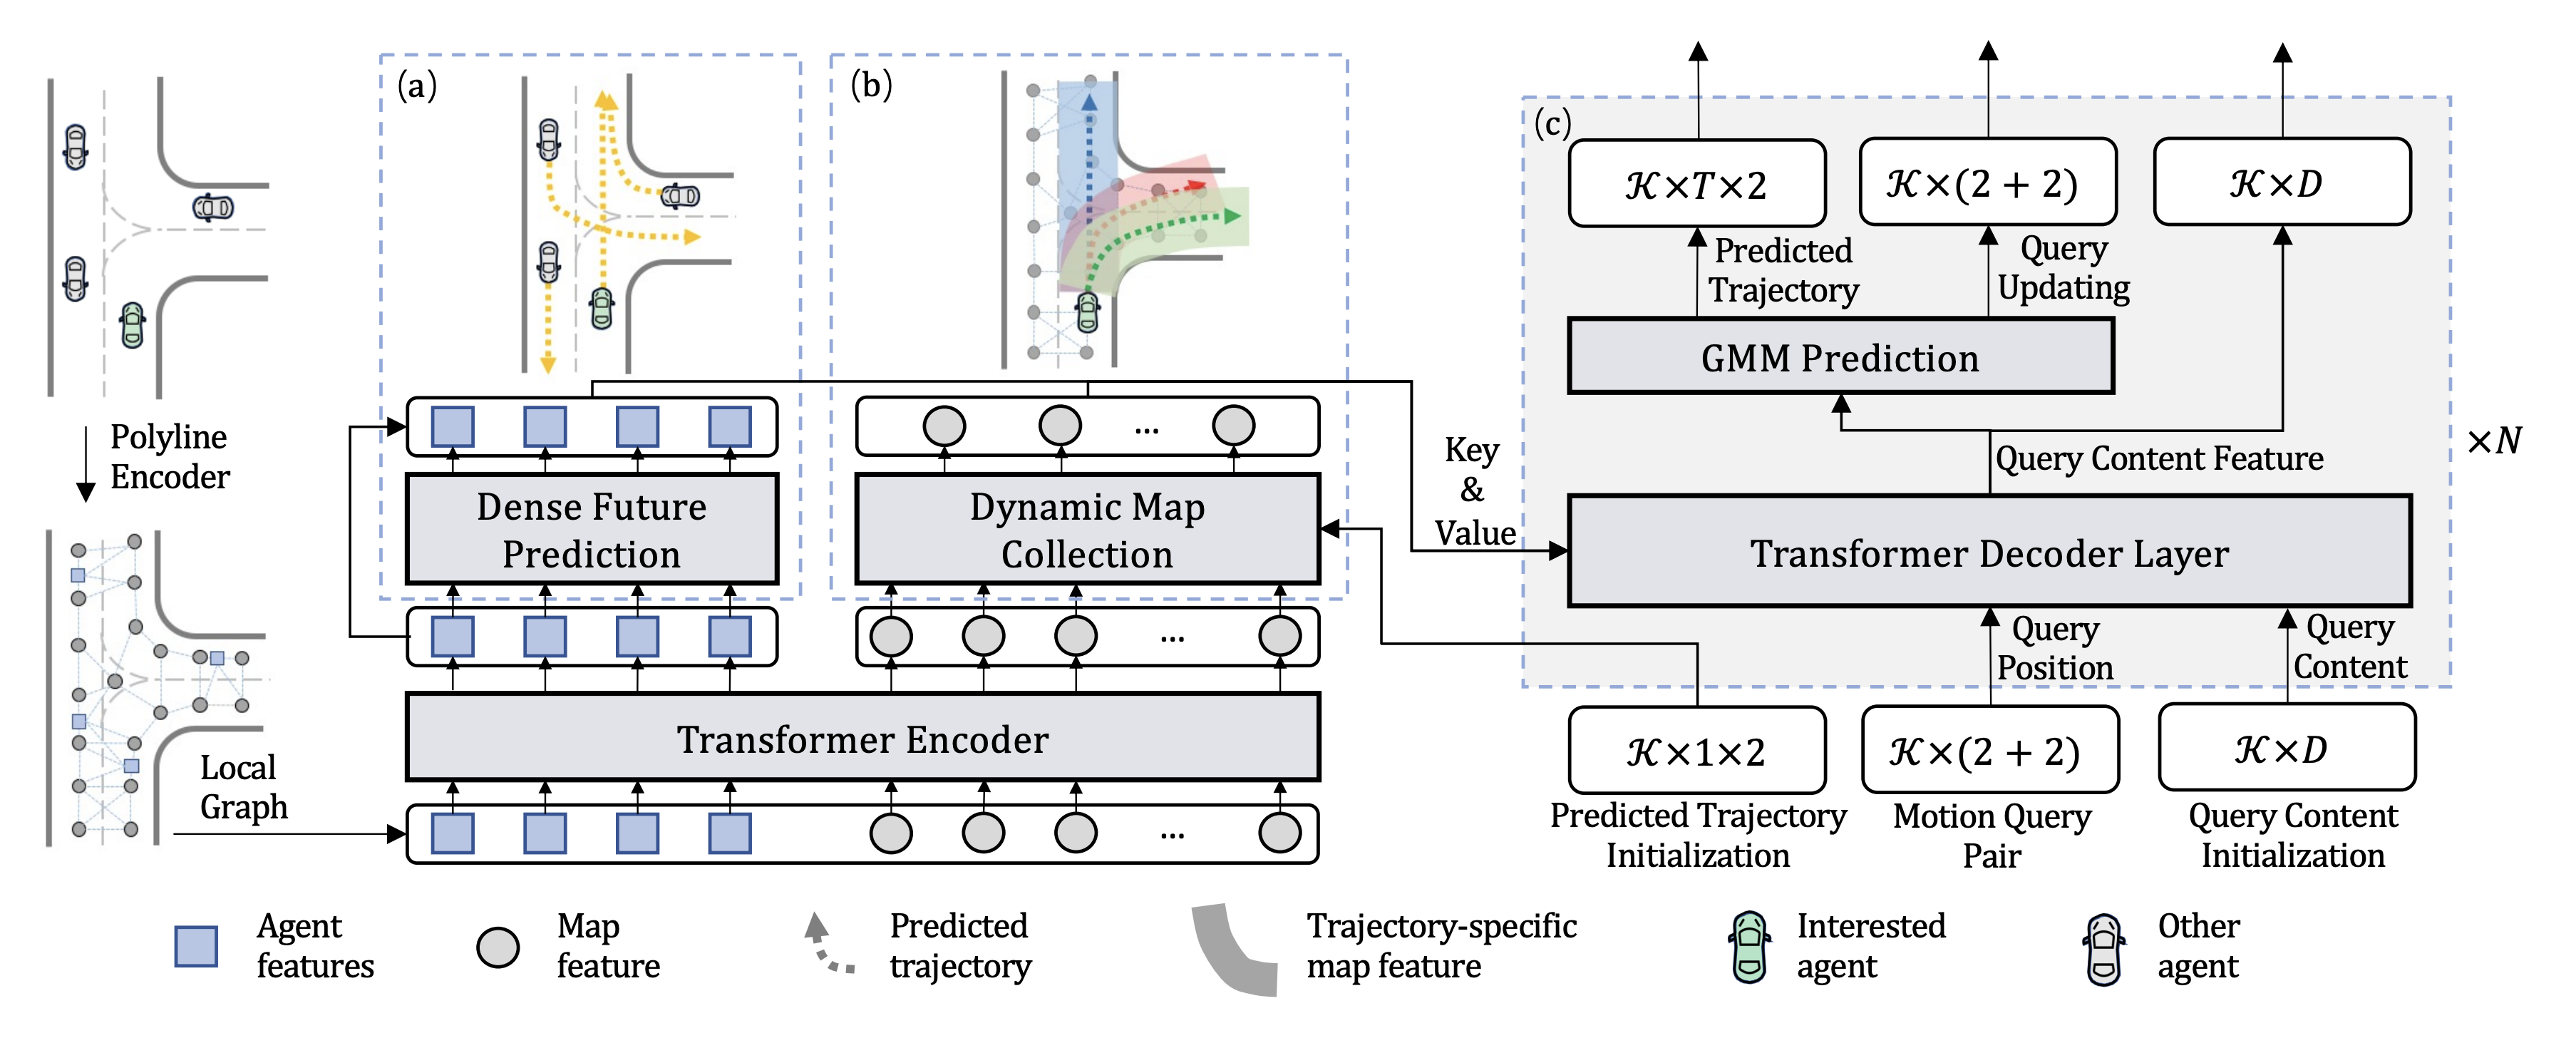
\includegraphics[width=0.85\textwidth]{docs/latex/figures/mtr_overall_architecture_detail.png}
        \caption{MTR architecture: A scene encoder builds context, and a motion decoder uses query pairs to generate multimodal trajectories~\cite{Shi2022MTR}.}
        \label{fig:mtr_architecture_pres}
    \end{figure}
\end{frame}

\begin{frame}{MTR: Input Encoding}
    MTR uses vectorized polylines for all scene elements, avoiding rasterization artifacts.
    \begin{columns}[T]
        \begin{column}{0.5\textwidth}
            \textbf{Map Elements}
            \begin{itemize}
                \item Lanes, boundaries, and crosswalks are represented as polylines.
                \item A PointNet-style MLP processes each polyline's points into a fixed-size feature vector.
                \item Max-pooling aggregates point features into a single polyline token.
            \end{itemize}
        \end{column}
        \begin{column}{0.5\textwidth}
            \textbf{Agent Histories}
            \begin{itemize}
                \item Past motion (position, heading, velocity) is also a polyline.
                \item Includes one-hot encodings for agent type (vehicle, pedestrian) and timestep.
                \item A similar MLP and pooling process creates an agent history token.
            \end{itemize}
        \end{column}
    \end{columns}
    \vfill
    \begin{block}{Scene Context Encoder}
        A Transformer encoder with \textbf{local self-attention} processes all map and agent tokens. Each element attends only to its $k$ nearest neighbors, efficiently building context-aware representations.
    \end{block}
\end{frame}

\begin{frame}{MTR Decoder: Motion Query Pairs}
    The decoder uses $K$ query pairs to generate $K$ trajectory modes. Each pair has a distinct role.
    \begin{columns}[T]
        \begin{column}{0.6\textwidth}
            \begin{itemize}
                \item\textbf{Static Intention Queries ($Q_I$):}
                \begin{itemize}
                    \item Act as stable anchors for different motion intentions (e.g., turn left, go straight).
                    \item Derived from clustering ground-truth trajectory endpoints.
                    \item Each query specializes in one high-level behavior, promoting prediction diversity.
                \end{itemize}
                \item\textbf{Dynamic Searching Queries ($Q_S$):}
                \begin{itemize}
                    \item Perform fine-grained path refinement.
                    \item At each decoder layer, the query is updated based on the previously predicted trajectory.
                    \item Probes the local scene context to make precise adjustments.
                \end{itemize}
            \end{itemize}
        \end{column}
        \begin{column}{0.4\textwidth}
            \begin{figure}
                \centering
                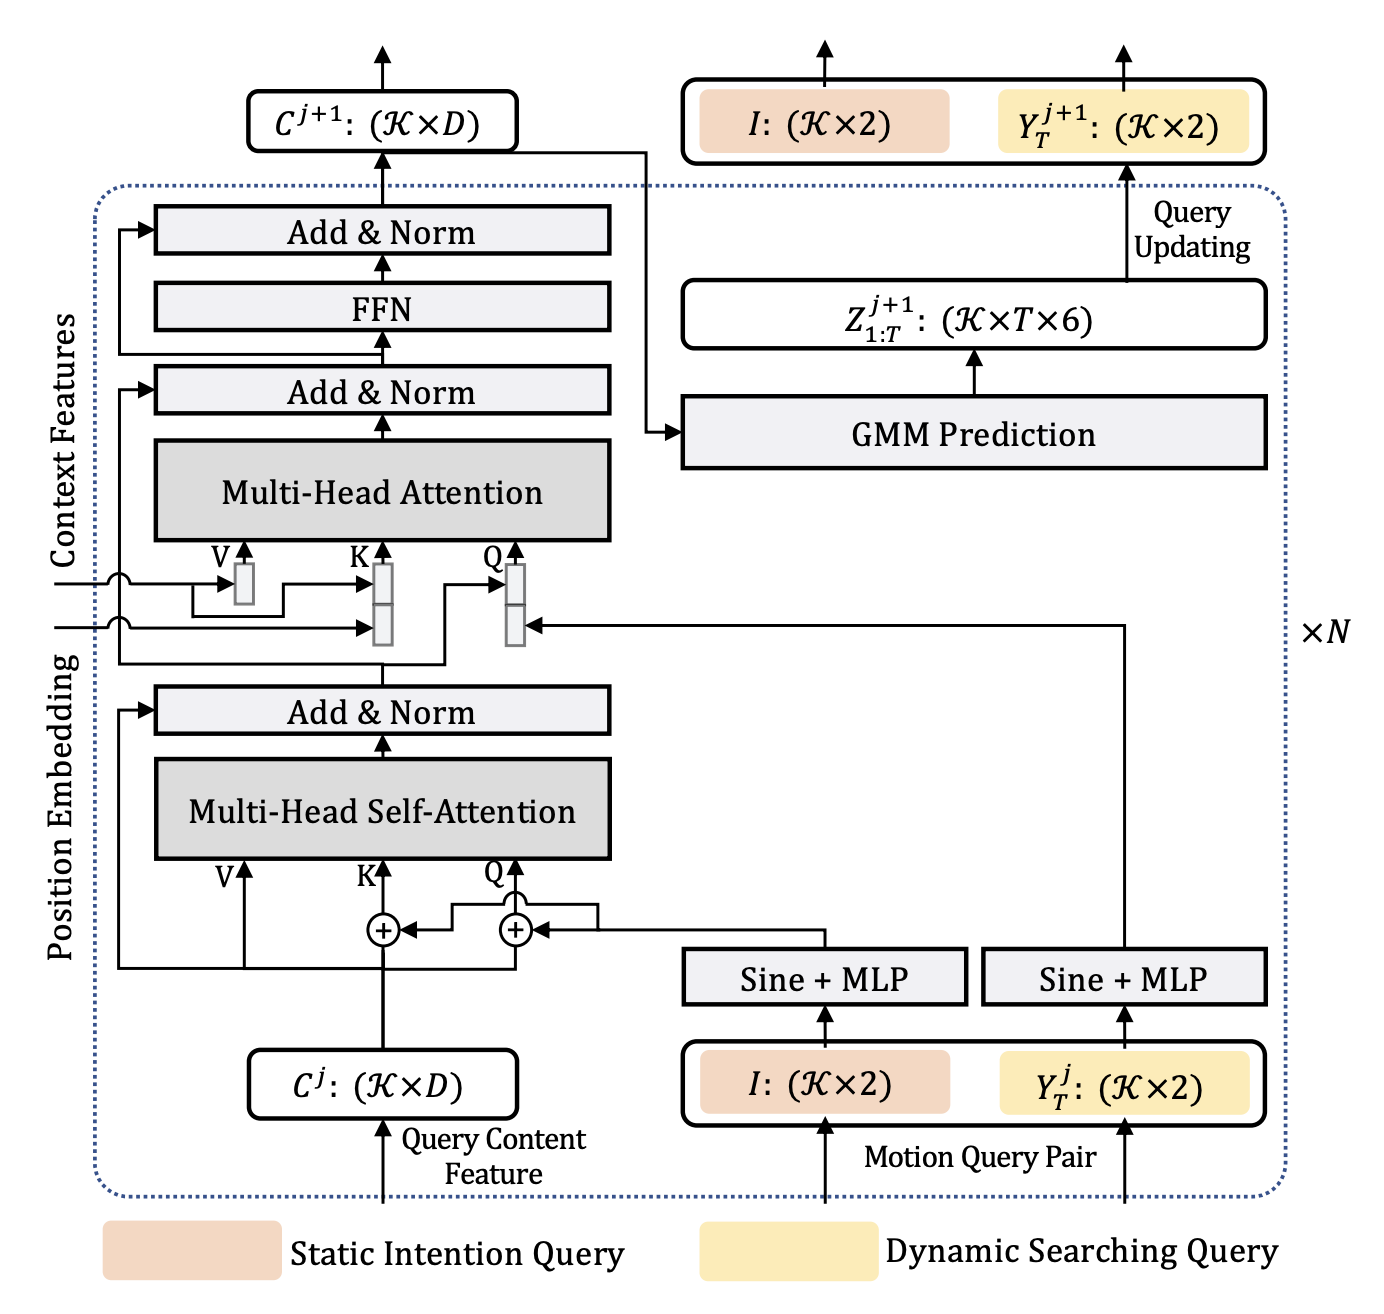
\includegraphics[width=0.9\textwidth]{docs/latex/figures/decoder_layer_detail.png}
                \caption{A single MTR decoder layer. The static query sets the goal, while the dynamic query refines the path iteratively~\cite{Shi2022MTR}}
            \end{figure}
        \end{column}
    \end{columns}
\end{frame}

\begin{frame}{MTR Decoder: Dynamic Map Collection}
    To ensure refinement is context-aware, the decoder focuses only on relevant map information.
    \begin{itemize}
        \item At each refinement step, the model identifies the $L$ map polylines closest to the current trajectory hypothesis.
        \item The dynamic query performs cross-attention only with these selected map features.
        \item This allows the model to ground its predictions in the immediate local geometry, such as staying within lane boundaries.
    \end{itemize}
    \begin{figure}
        \centering
        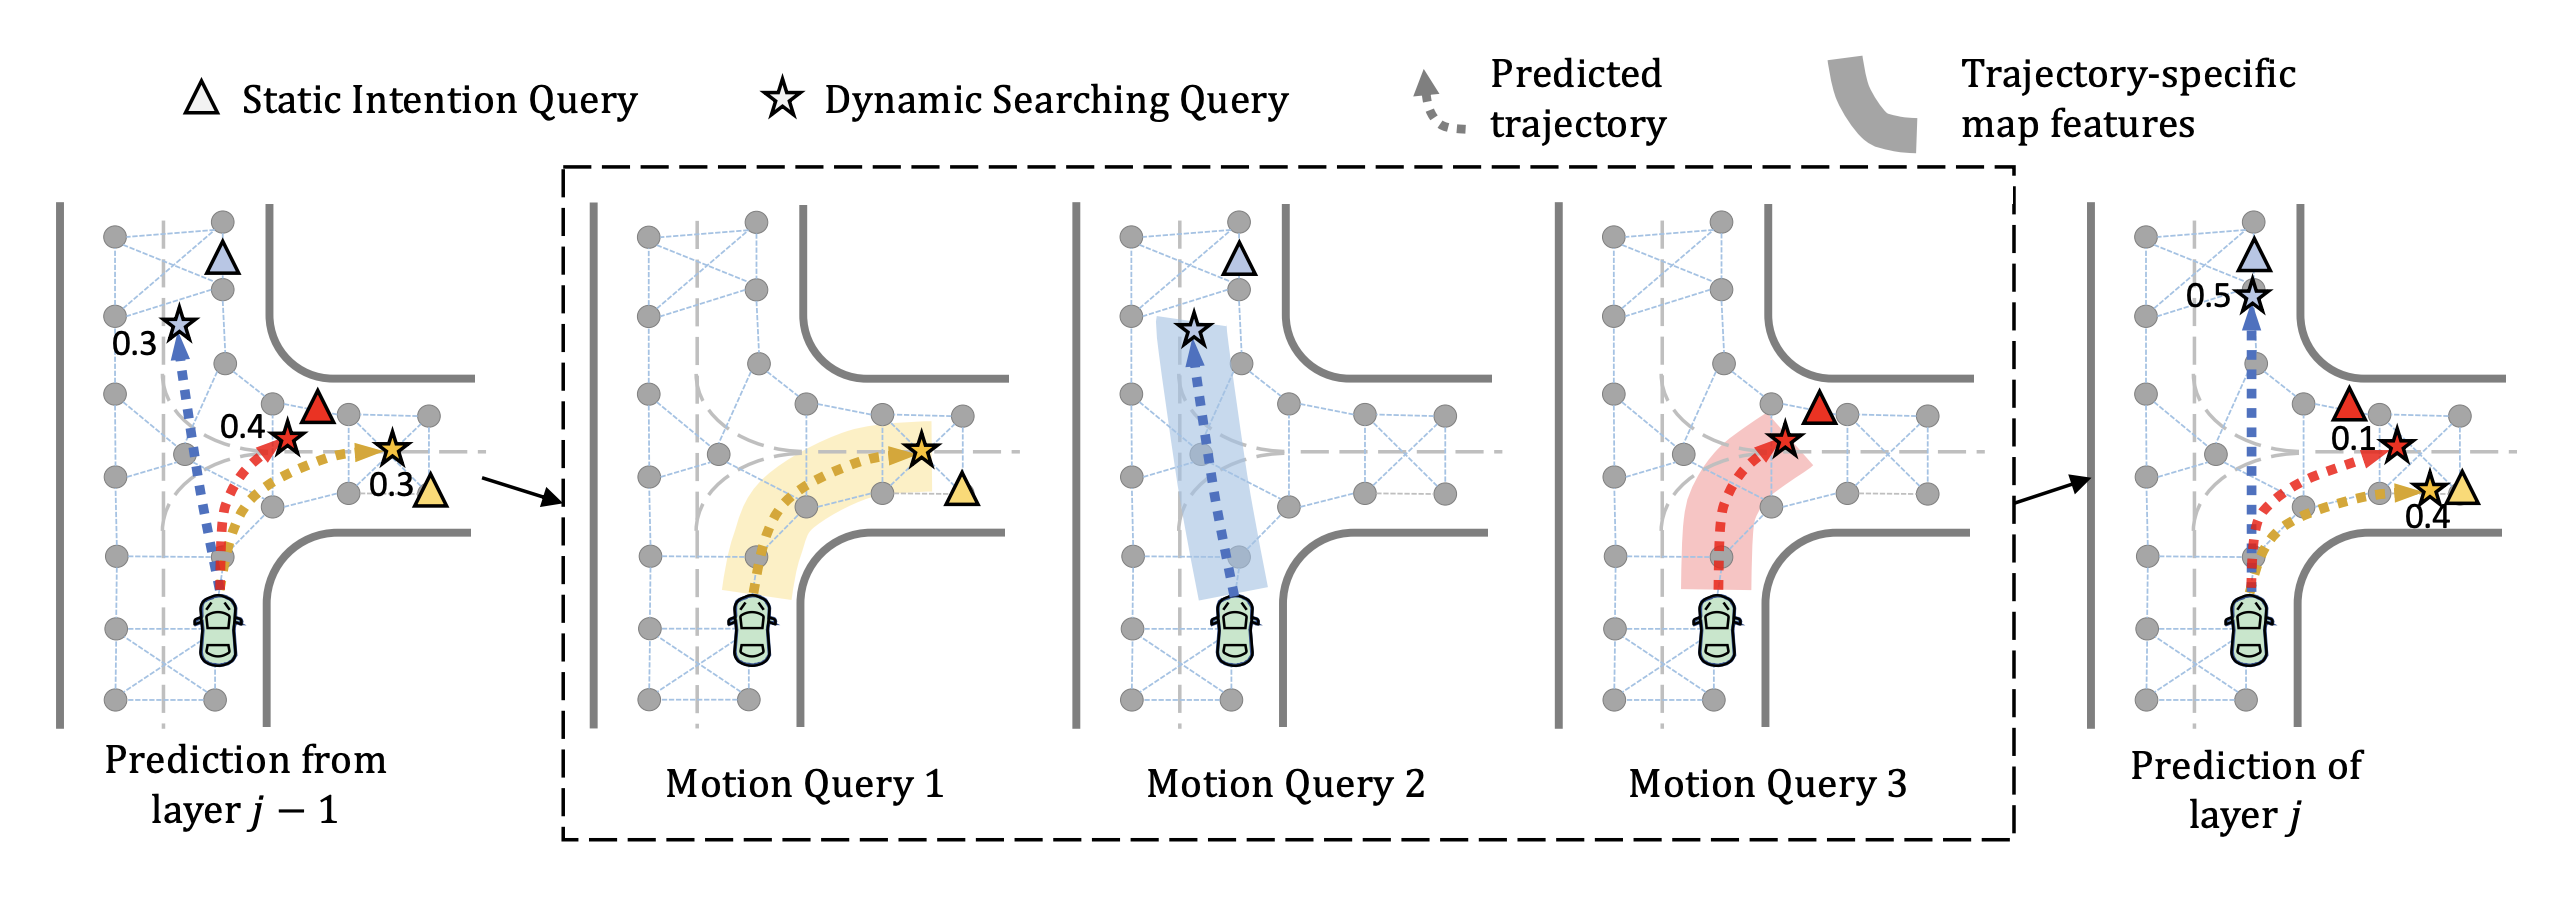
\includegraphics[width=0.7\textwidth]{docs/latex/figures/dynamic_map.png}
        \caption{As the trajectory is refined (dashed line), the decoder dynamically selects the closest map polylines (highlighted) to inform the next step~\cite{Shi2022MTR}.}
        \label{fig:dynamic_map_pres}
    \end{figure}
\end{frame}

\begin{frame}{MTR: Input-Output Formulation}
    \begin{columns}[T]
        \begin{column}{0.5\textwidth}
            \textbf{Input Domain}
            \begin{itemize}
                \item \textbf{Agent of Interest:} Historical trajectory (position, velocity, heading).
                \item \textbf{Context Agents:} Histories of surrounding agents.
                \item \textbf{Map Features:} Vectorized polylines for lanes, crosswalks, etc.
                \item All inputs are transformed into the agent-of-interest's local coordinate system.
            \end{itemize}
        \end{column}
        \begin{column}{0.5\textwidth}
            \textbf{Output Domain}
            \begin{itemize}
                \item A set of $K$ probable future trajectories (e.g., $K=64$).
                \item Each trajectory is a sequence of waypoints over a future time horizon (e.g., 8s).
                \item Each trajectory is assigned a confidence score $p_k$.
                \item This forms a Gaussian Mixture Model (GMM) representing the prediction distribution.
            \end{itemize}
        \end{column}
    \end{columns}
    \vfill
    \begin{block}{Key Transformation}
        MTR transforms historical, agent-centric scene vectors into a ranked, multimodal distribution of future paths.
    \end{block}
\end{frame}

\begin{frame}{MTR: Training and Loss Function}
    The model is trained using a "winner-takes-all" strategy that combines classification and regression losses.
    \begin{itemize}
        \item \textbf{1. Find the Best Match:} For each training example, the model finds the predicted trajectory $\mathcal{T}_k$ that is closest to the ground-truth trajectory $\mathcal{T}_{gt}$. This is the "winning" prediction.
        \item \textbf{2. Classification Loss:} A classification loss (e.g., cross-entropy) encourages the model to assign a high probability $p_k$ to this winning mode.
        \item \textbf{3. Regression Loss:} A regression loss (e.g., L1 or L2 distance) penalizes the waypoint differences between the winning trajectory $\mathcal{T}_k$ and the ground truth $\mathcal{T}_{gt}$.
    \end{itemize}
    \begin{equation}
        \mathcal{L}_{\text{total}} = \mathcal{L}_{\text{cls}}(p_k, \text{winner}) + \alpha \cdot \mathcal{L}_{\text{reg}}(\mathcal{T}_k, \mathcal{T}_{gt})
    \end{equation}
    \begin{alertblock}{Supervision Strategy}
        This loss is applied at \emph{every} layer of the decoder, encouraging iterative refinement from a coarse guess to a fine-grained path.
    \end{alertblock}
\end{frame}

\begin{frame}{MTR: Quantitative Results}
    \begin{block}{Performance on Agrovere 2 Dataset}
        Our trained MTR model was evaluated against the official paper results on the validation set.
    \end{block}
    \begin{table}
        \centering
        \renewcommand{\arraystretch}{1.3}
        \begin{tabular}{|l|c|c|c|}
            \hline
            \textbf{Metric} & \textbf{Our Model} & \textbf{Paper Results} & \textbf{Improvement} \\
            \hline
            brier-minFDE ($\uparrow$) & \textbf{1.98} & 2.08 & \textcolor{mygreen}{-4.8\%} \\
            minFDE@1 ($\uparrow$) & \textbf{1.67} & 1.68 & \textcolor{mygreen}{-0.6\%} \\
            minADE@1 ($\downarrow$) & 0.86 & \textbf{0.85} & \textcolor{myred}{+1.2\%} \\
            Miss Rate@1 ($\downarrow$) & 0.3014\% & \textbf{0.3\%} & \textcolor{myred}{+0.5\%} \\
            \hline
        \end{tabular}
        \caption{Comparison of key performance metrics.}
    \end{table}
    \begin{alertblock}{Key Takeaway}
        The model significantly improves the brier-minFDE score, indicating better-calibrated uncertainty estimates alongside competitive trajectory accuracy.
    \end{alertblock}
\end{frame}

\begin{frame}{MTR: Use Case - Vehicle at Crosswalk}
    Consider a vehicle (1) turning right while a pedestrian (2) is on a crosswalk.
    \begin{columns}[T]
        \begin{column}{0.4\textwidth}
            \begin{figure}
                \centering
                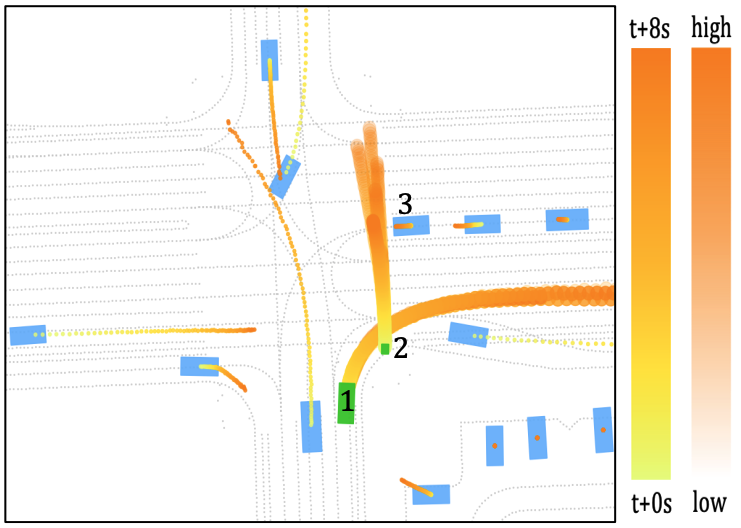
\includegraphics[width=0.95\textwidth]{docs/latex/figures/input_output_viz_crosswalk_detail.png}
                \caption{MTR's prediction for a vehicle (1) turning right. The model correctly identifies yielding to the pedestrian (2) as the most likely outcome.}
            \end{figure}
        \end{column}
        \begin{column}{0.6\textwidth}
            \textbf{Input Relations:}
            \begin{itemize}
                \item The model encodes the history of the turning vehicle (1, green) and the pedestrian (2, blue).
                \item Map polylines for the crosswalk and lane boundaries are also encoded.
                \item The encoder's attention mechanism fuses these inputs, capturing the critical vehicle-pedestrian interaction.
            \end{itemize}
            \textbf{Output Relations:}
            \begin{itemize}
                \item The model generates multiple future trajectories (orange/yellow).
                \item The most probable mode shows the vehicle waiting for the pedestrian to pass before completing the turn.
                \item The high confidence in this yielding maneuver shows the model's ability to produce socially compliant predictions.
            \end{itemize}
        \end{column}
    \end{columns}
\end{frame}
% conclusion: MTR effectively disentangles multimodality by using static queries for high-level intentions and dynamic queries for detailed path refinement.


%==============================================================================
% LMFormer Section
%==============================================================================
\subsection{LMFormer: A Query-Centric Approach}

\begin{frame}{LMFormer: A Query-Centric Approach}
    \begin{columns}[T]
        \begin{column}{0.5\textwidth}
            \textbf{Key Features:}
            \begin{itemize}
                \item Fully query-centric: end-to-end \(\mathrm{SE}(2) \rtimes \mathbb{R} \times S_n\) invariance.
                \item Factorized attention to model relationships between all scene elements.
                \item Two-level recurrent decoder for iterative, coarse-to-fine refinement of autoregressively generated motion vectors.
            \end{itemize}
        \end{column}
        \begin{column}{0.5\textwidth}
            \begin{figure}
                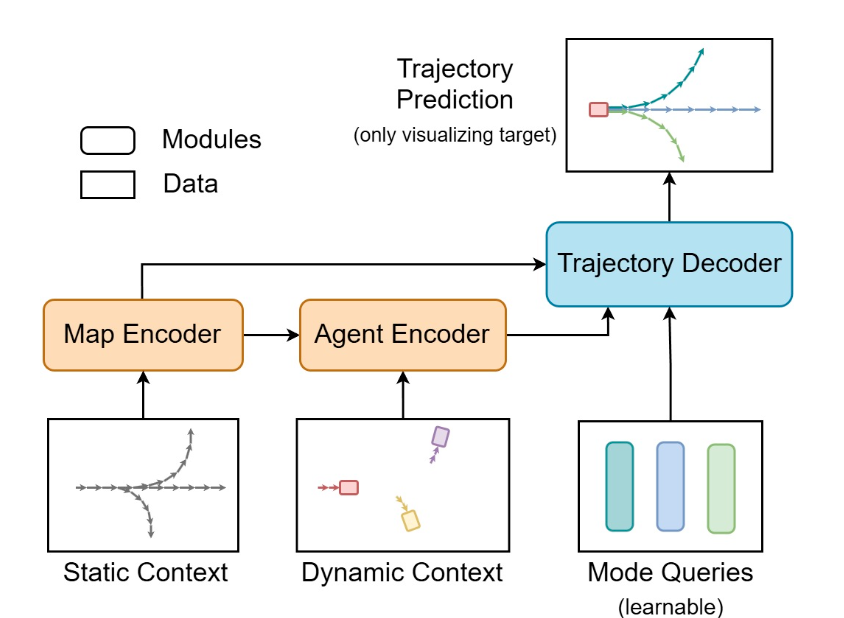
\includegraphics[width=\textwidth]{docs/figures/lmformer_arch.png}
                \caption{LMFormer architecture overview~\cite{lmformerYadav2025}.}
            \end{figure}
        \end{column}
    \end{columns}
\end{frame}

\begin{frame}{LMFormer: Encoder Architecture}
    \begin{columns}[T]
        \begin{column}{0.5\textwidth}
            \textbf{Encoder Modules:}
            \begin{itemize}
                \item \textbf{Learnable Fourier Embeddings}: Lifts all scalar inputs (geometry, kinematics) to a high-frequency space.
                \item \textbf{Lane Encoder}: Captures static map topology with self-attention over lane segments.
                \item \textbf{Agent Encoder}: Models dynamic context via three stacked attention layers:
                    \begin{itemize}
                        \item Temporal Self-Attention
                        \item Agent-Agent Cross-Attention
                        \item Agent-Lane Cross-Attention
                    \end{itemize}
            \end{itemize}
        \end{column}
        \begin{column}{0.5\textwidth}
            \begin{figure}
                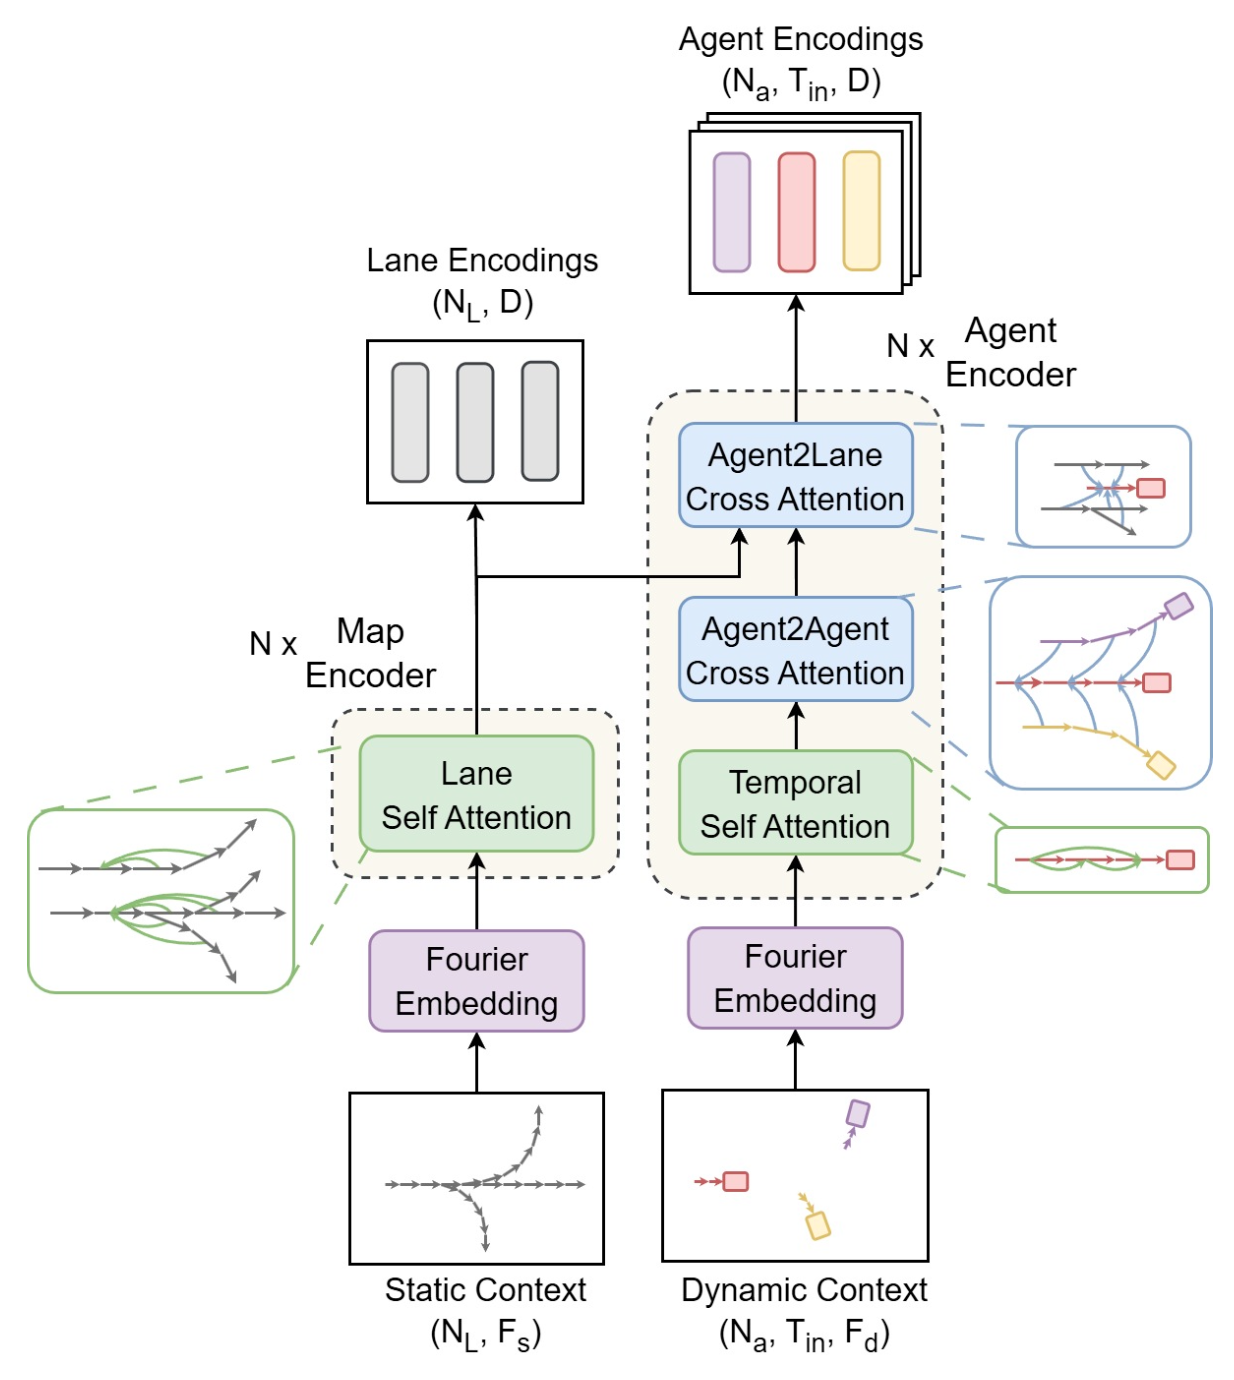
\includegraphics[width=\textwidth, height=0.7\textheight, keepaspectratio]{docs/figures/lmformer_arch_encorder.png}
                \caption{Detailed view of the LMFormer encoder modules~\cite{lmformerYadav2025}.}
            \end{figure}
        \end{column}
    \end{columns}
\end{frame}

\begin{frame}{Encoder: Learnable Fourier Embeddings}
  \begin{columns}[T]
    \column{0.6\textwidth}
      \begin{itemize}
        \item All scalar inputs (lane geometry, motion history) are lifted with \textbf{learnable Fourier features}~\cite{li2021llearnableFourier}.
        \item This allows the model to learn spatio-temporal patterns at various, task-adaptive frequencies.
      \end{itemize}
      \begin{equation}
        \label{eq:pres_learnable_fourier_embedding}
        \mathbf{x} \mapsto \text{GeLU}\!\bigl(\mathbf{W}_A [\sin(2\pi \mathbf{x}\mathbf{W}_f^T)\oplus\cos(2\pi \mathbf{x}\mathbf{W}_f^T)] + \mathbf{B}_\varphi\bigr) + \mathbf{B}_\psi
      \end{equation}
      \begin{itemize}
        \item[\(\mathbf{W}_f\)] learns which harmonic frequencies to emphasize.
        \item[\(\mathbf{W}_A\)] learns the amplitude of each frequency.
        \item[\(\mathbf{B}_\varphi\)] are learnable phase shifts.
        \item[\(\mathbf{B}_\psi\)] are learnable biases.
      \end{itemize}
      \vspace{1em}
      \small{The learnable basis adapts to capture the most informative spatio-temporal frequencies for the prediction task.}

    \column{0.38\textwidth}
      \begin{figure}
        \centering
        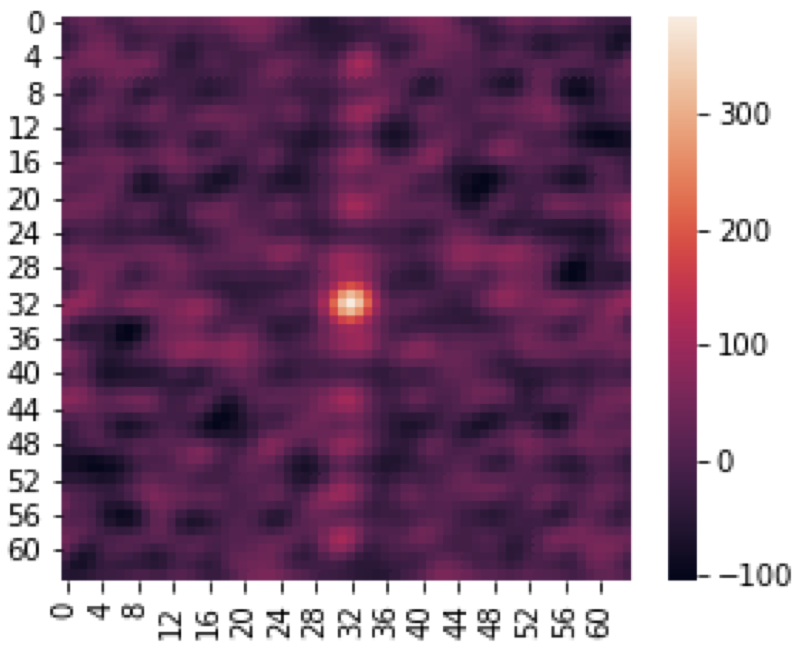
\includegraphics[width=\columnwidth,height=0.25\textheight,keepaspectratio]{docs/latex/figures/lff_high_freq.png}
        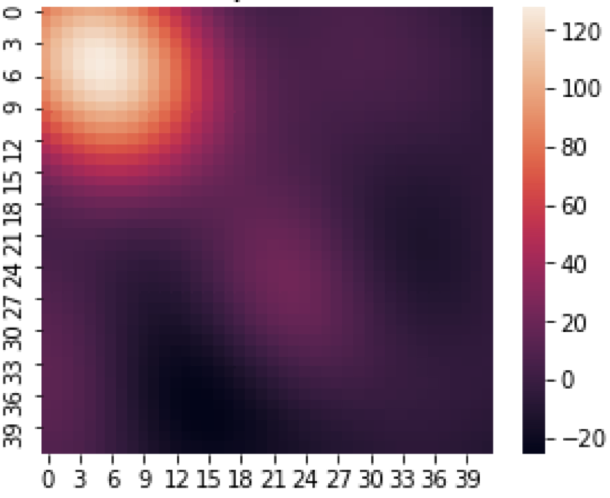
\includegraphics[width=\columnwidth,height=0.25\textheight,keepaspectratio]{docs/latex/figures/lff_low_freq_ball.png}
        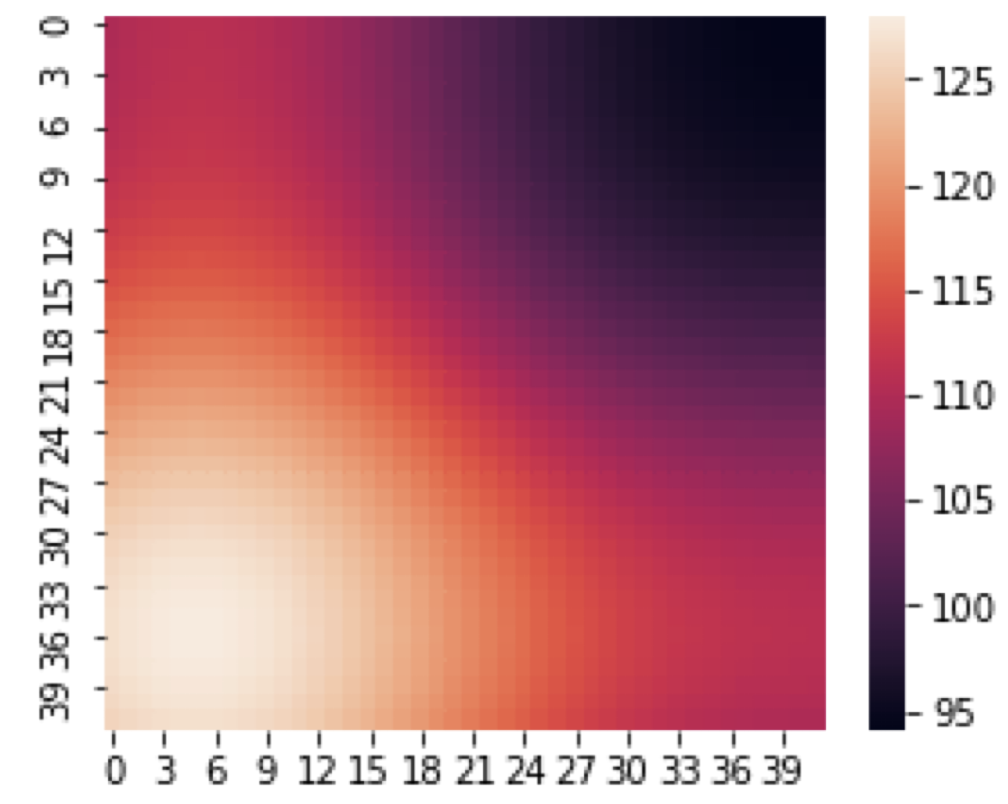
\includegraphics[width=\columnwidth,height=0.25\textheight,keepaspectratio]{docs/latex/figures/lff_low_freq_diag.png}
        \caption{LFF captures different harmonics~\cite{li2021llearnableFourier}.}
      \end{figure}
  \end{columns}
\end{frame}

\begin{frame}{Encoder: Attention Mechanisms}
  \begin{columns}[T]
    \column{0.6\textwidth}
      \begin{itemize}
        \item<1-> \textbf{Map (Lane) Encoder:}\\
          Applies self-attention over lane-segment tokens to capture topology and geometry.\\
          Result: Static scene encodings \(\mathbf{E}_s \in \mathbb{R}^{N_{\text{map}} \times D}\).
        \item<2-> \textbf{Agent Encoder:} Stacks three attention modules:
          \begin{enumerate}[<+->]
            \item Temporal self-attention (agent's own past).
            \item Agent-agent cross-attention (social interactions).
            \item Agent-lane cross-attention (grounding in map).
          \end{enumerate}
          Result: Agent encodings \(\mathbf{E}_d \in \mathbb{R}^{N_{A} \times T_{p} \times D}\).
      \end{itemize}

    \column{0.35\textwidth}
      % Lane self-attention (always visible)
      \only<1->{%
        \centering
        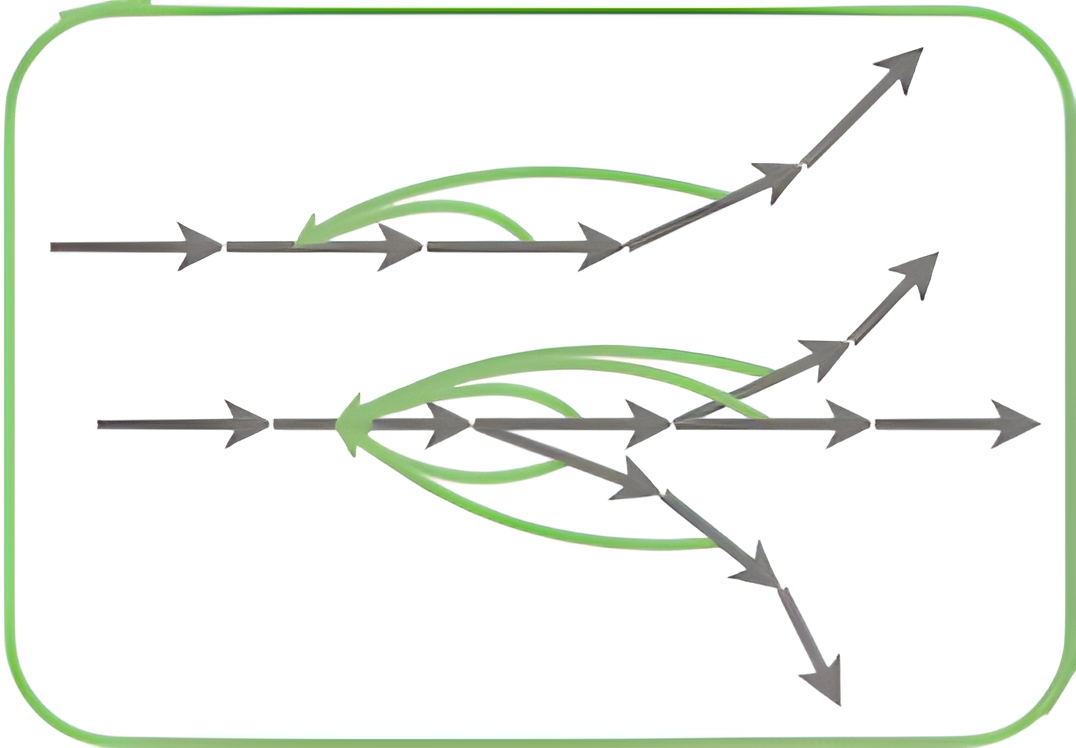
\includegraphics[width=\columnwidth,height=0.25\textheight,keepaspectratio]{docs/latex/figures/a-sa-l2l.png}
      }
  \end{columns}
    \only<2->{%
        \centering
        \begin{figure}
        \centering
        \begin{tabular}{ccc}
          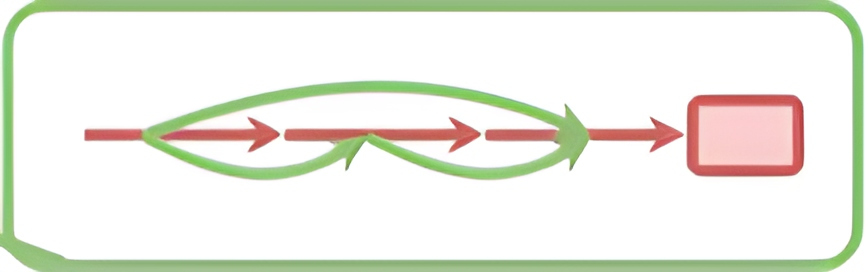
\includegraphics[width=0.32\columnwidth,height=0.25\textheight,keepaspectratio]{docs/latex/figures/a-sa-a2t.png} &
          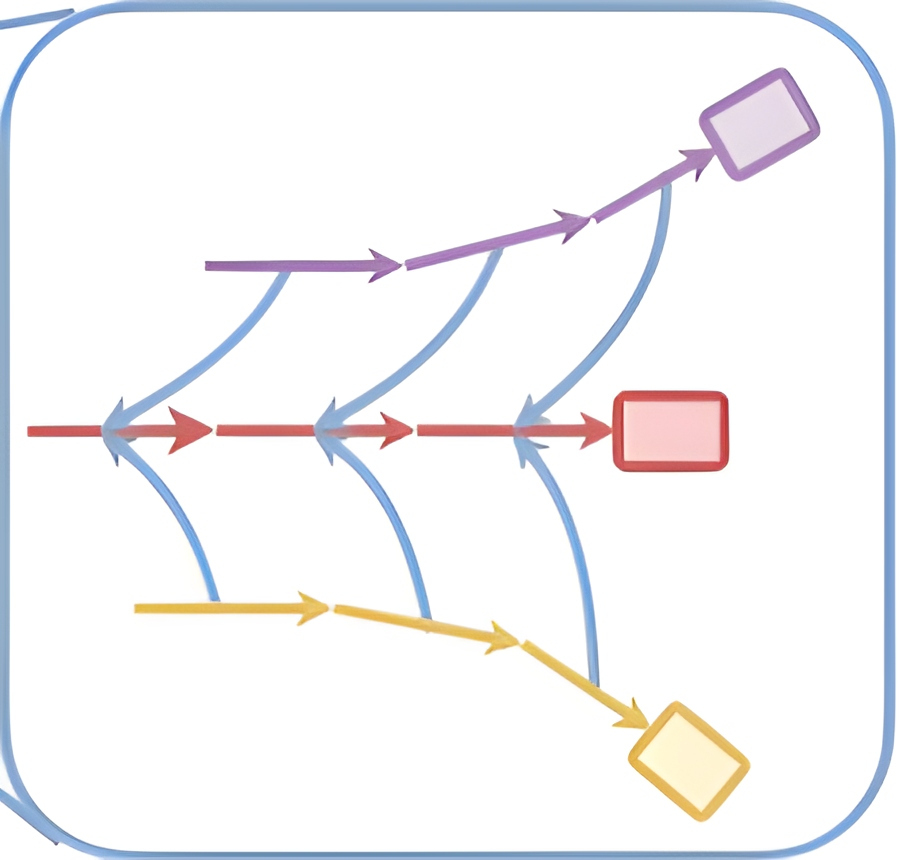
\includegraphics[width=0.32\columnwidth,height=0.25\textheight,keepaspectratio]{docs/latex/figures/a-ca-a2a.png} &
          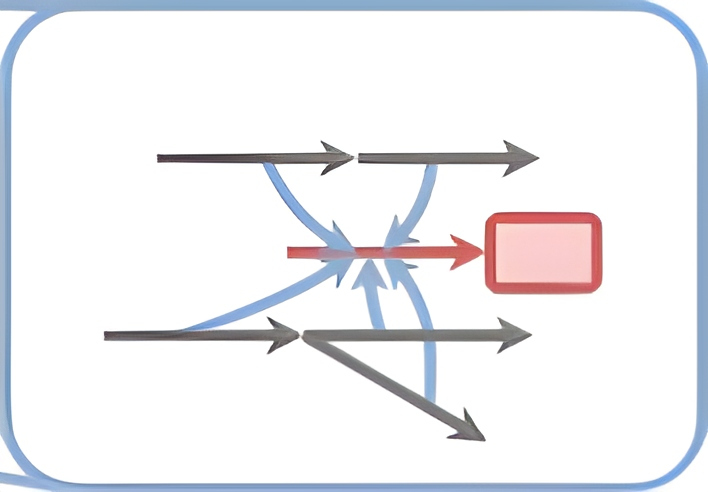
\includegraphics[width=0.32\columnwidth,height=0.25\textheight,keepaspectratio]{docs/latex/figures/a-ca-a2l.png}
        \end{tabular}
        \caption{Attention mechanisms in the agent encoder: Temporal, Agent, and Lane cross-attention~\cite{lmformerYadav2025}.}
        \end{figure}
      }
\end{frame}

\begin{frame}{LMFormer: Decoder Architecture}
    \begin{columns}[T]
        \begin{column}{0.5\textwidth}
            \textbf{Decoder Features:}
            \begin{itemize}
                \item \textbf{Iterative Refinement}: Inspired by DAB-DETR~\cite{liu2022dabdetr}, coarse-to-fine trajectory generation across \(N_{\text{dec}}\) layers.
                \item \textbf{Three Cross-Attention Types}:
                    \begin{itemize}
                        \item Mode2Temporal (temporal dependencies-per agent)
                        \item Mode2Agent (social interactions-between agents)
                        \item Mode2Lane (map grounding)
                    \end{itemize}
                \item \textbf{Autoregressive Generation}: Future motion vectors generated sequentially over \(T_f\) timesteps (independently in each layer).
                \item \textbf{Bottleneck Design}: Only final timestep passed to next layer to create a bottleneck.
                \item \textbf{MLP Output}: Motion vectors with uncertainty from refined queries as \emph{Laplacian Mixture Models}.
            \end{itemize}
        \end{column}
        \begin{column}{0.5\textwidth}
            \begin{figure}
                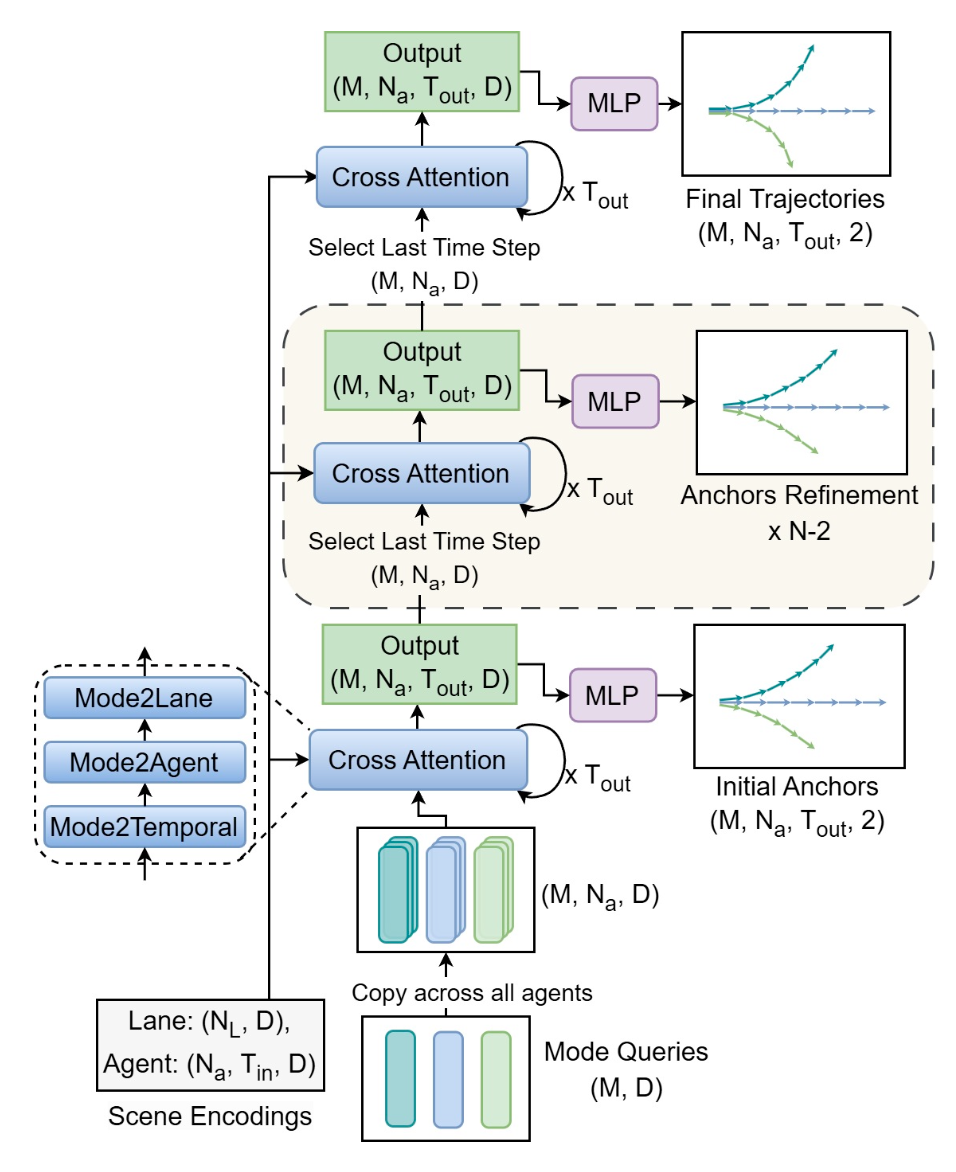
\includegraphics[width=\textwidth, height=0.7\textheight, keepaspectratio]{docs/figures/lmformer_arch_decoder.png}
                \caption{LMFormer decoder with recurrent cross-attention modules~\cite{lmformerYadav2025}.}
            \end{figure}
        \end{column}
    \end{columns}
\end{frame}

\begin{frame}[fragile]{Decoder: Recurrent Cross-Attention}
    \begin{block}{LMFormer Recurrent Cross-Attention Decoder}
    \begin{algorithmic}[1]
    \footnotesize
    \Require Agent encodings \(\mathbf{E}_d \in \mathbb{R}^{N \times T_{p} \times D}\), Lane encodings \(\mathbf{E}_s \in \mathbb{R}^{N_L \times D}\), Learned Mode anchors \(\mathbf{A} \in \mathbb{R}^{M \times D}\)
    \Ensure Trajectory sets \(\{\mathcal{T}_{out}^{(i)}\}_{i=1}^{N_{\text{dec}}}\)
    \State \(\mathbf{q} \leftarrow \text{repeat}(\mathbf{A}, N)\) \(\triangleright\) Initialize mode queries \((M, N, D)\)
    \For{\(i = 1\) \textbf{to} \(N_{\text{dec}}\)}
        \State \(\mathbf{Q}_{\text{seq}}^{(i)} \leftarrow \text{zeros}(M, N, T_f, D)\)
        \For{\(t = 1\) \textbf{to} \(T_f\)}
            \State \(\triangleright\) \textbf{Mode2Temporal}
            \State \(\mathbf{q}\leftarrow \text{CrossAttn}(\mathbf{q}, K=V=\mathbf{E}_d[\text{same } n, \tau=1\dots T_p, :])\)
            \State \(\triangleright\) \textbf{Mode2Agent}
            \State \(\mathbf{q}\leftarrow \text{CrossAttn}(\mathbf{q}, K=V=\mathbf{E}_d[\tilde{n}=1\dots N, \text{same }\tau, :])\)
            \State \(\triangleright\) \textbf{Mode2Lane}
            \State \(\mathbf{q}\leftarrow \text{CrossAttn}(\mathbf{q}, K=V=\mathbf{E}_s)\)
            \State \(\mathbf{Q}_{\text{seq}}^{(i)}[:,:,t,:] \leftarrow \mathbf{q}\)
        \EndFor
        \State \(\mathcal{T}_{out}^{(i)} \leftarrow \text{MLP}(\mathbf{Q}_{\text{seq}}^{(i)})\) \(\triangleright\) \((M, N, T_f, 4)\)
    \EndFor
    \end{algorithmic}
    \end{block}
\end{frame}

\begin{frame}{Decoder: Output and Loss}
    \textbf{Output Formulation}
    \begin{itemize}
        \item Every mode query predicts a \textbf{motion-vector chain}:
    \end{itemize}
    \begin{equation}
    \mathcal{T}_{out}^{a,m} = \bigl[(V_1^{a,m},S_1^{a,m}),\dots,(V_{T_f}^{a,m},S_{T_f}^{a,m})\bigr], \quad V_\bullet^{a,m}, S_\bullet^{a,m} \in \mathbb{R}^2
    \end{equation}
    where \(V_t\) is a displacement vector and \(S_t\) its uncertainty, parameterizing a Laplacian mixture.

    \vspace{1em}
    \textbf{Loss Formulation}
    \begin{itemize}
        \item Combines winner-takes-all regression loss and classification loss-same as MTR but with LMM instead of GMM.
        \item Supervises all but the first refinement layer to encourage coarse-to-fine refinement.
    \end{itemize}

    \begin{equation}
    \mathcal{L}
    = \lambda\,\mathcal{L}_{cls}
        + \sum_{n=2}^{N_{\text{dec}}}\mathcal{L}_{reg}^{(n)},
    \label{eq:lm_loss}
    \end{equation}
\end{frame}

\begin{frame}{LMFormer: Qualitative Comparison}
    \begin{columns}[T]
        \begin{column}{0.5\textwidth}
            \textbf{Pros} \greenoplus
            \begin{itemize}
                \item Fully query-centric (\(\mathrm{SE}(2)\) invariant).
                \item Joint multi-agent decoding.
                \item Temporally coherent refinement.
                \item Reduced VRAM vs. QCNet.
            \end{itemize}
        \end{column}
        \begin{column}{0.5\textwidth}
            \textbf{Cons} \redominus
            \begin{itemize}
                \item High VRAM vs. CASPFormer.
                \item Lane-only static context.
                \item Uniform loss weighting.
                \item Generalization challenges.
            \end{itemize}
        \end{column}
    \end{columns}
\end{frame}

\section{Conclusion}

\begin{frame}[plain]
  \begin{center}
    \vfill
    {\Huge \textbf{Conclusion}}
    \vfill
    {\Large Synthesis and Reflection}
    \vfill
  \end{center}
\end{frame}

\subsection{A Qualitative Comparison of the Selected Architectures}

\begin{frame}{Relation to CASPNet \& CASPFormer}
    \begin{itemize}
        \item \textbf{CASPNet}: Operates on raster grids, predicts per-pixel occupancies.
        \item \textbf{CASPFormer}: Adds deformable attention and vector outputs but remains \emph{agent-centric}.
        \item \textbf{LMFormer}: Discards the raster backbone entirely for a \emph{query-centric} paradigm.
    \end{itemize}
    \vfill
    \begin{alertblock}{Key Trade-off}
    Gains strict symmetry compliance and parallel multi-agent decoding at the cost of a larger key-value cache and higher VRAM demand (\(\approx\)2x CASPFormer).
    \end{alertblock}
\end{frame}


%==============================================================================
% Comparative Analysis
%==============================================================================
\subsection{Comparative Analysis}

\begin{frame}{Comparative Analysis of Architectures}
    \begin{table}
    \centering
    \tiny
    \renewcommand{\arraystretch}{1.2}
    \begin{tabular}{|p{1.9cm}|p{3.9cm}|p{3.9cm}|p{3.9cm}|}
        \hline
        \textbf{Aspect} & \textbf{CASPFormer (Raster-Centric)} & \textbf{MTR (Hybrid)} & \textbf{LMFormer (Query-Centric)} \\
        \hline
        \textbf{Scene Representation} & Rasterized BEV grids. & Vectorized polylines. & Vectorized polylines. \\
        \hline
        \textbf{Coordinate System} & Agent-centric (ego frame). & Agent-centric (target frame). & Query-centric (local frames). \\
        \hline
        \textbf{Symmetry} & No inherent symmetries for context agents. & Invariant for target agent only. & Full SE(2) \(\times\) \(\mathbb{R}\) invariance. \\
        \hline
        \textbf{Encoder} & CNN backbone with FPN. & PointNet-style MLP + Transformer with local attention. & Transformer with learnable Fourier features. \\
        \hline
        \textbf{Decoder} & Deformable cross-attention on multi-scale feature maps. & Motion query pairs (static intention + dynamic search). & Recurrent cross-attention on mode queries. \\
        \hline
        \textbf{Pros} \greenoplus &
        \begin{itemize}
            \item Efficient Transformer decoding.
            \item Direct vectorized output.
            \item Explicit uncertainty estimates.
        \end{itemize} &
        \begin{itemize}
            \item High geometric precision.
            \item Interpretable query-based modes.
            \item Dynamic map attention.
        \end{itemize} &
        \begin{itemize}
            \item Fully SE(2) invariant.
            \item Joint multi-agent decoding.
            \item Temporally coherent refinement.
        \end{itemize} \\
        \hline
        \textbf{Cons} \redominus &
        \begin{itemize}
            \item Inherits raster artifacts.
            \item Limited to ego-centric view.
            \item Quadratic scaling in encoder.
        \end{itemize} &
        \begin{itemize}
            \item Requires NMS post-processing.
            \item Intention queries may miss rare maneuvers.
            \item Lacks explicit physical constraints.
        \end{itemize} &
        \begin{itemize}
            \item High VRAM demand.
            \item Lane-only static context.
            \item Generalization challenges.
        \end{itemize} \\
        \hline
    \end{tabular}
    \end{table}
    \begin{alertblock}{Architectural Trade-off}
        The field is moving from raster-based, agent-centric models (CASPFormer) towards fully vectorized, query-centric paradigms (LMFormer). This shift trades CNN simplicity for the geometric precision and symmetry of Transformers, at the cost of higher memory. MTR represents a hybrid approach, combining a vectorized but agent-centric encoder with a query-based decoder.
    \end{alertblock}
\end{frame}


%==============================================================================
% Conclusion
%==============================================================================
\section{Project Conclusion}

\begin{frame}{Summary of Achievements}
    \begin{columns}[T]
        \begin{column}{0.6\textwidth}
            \textbf{Theoretical Contributions}
            \begin{itemize}
                \item Conducted a deep comparative analysis of trajectory prediction architectures, from raster-based (CASPNet) to modern query-centric Transformers (MTR, LMFormer).
                \item Deconstructed the agent-centric vs. query-centric paradigms, highlighting the role of symmetry and invariance ($\mathrm{SE}(2)$) in building robust models.
                \item Analyzed key architectural features for multimodality, including motion query pairs and recurrent refinement.
            \end{itemize}
        \end{column}
        \begin{column}{0.4\textwidth}
            \textbf{Practical Contributions}
            \begin{itemize}
                \item Refactored and modernized the UniTraj framework for robust experimentation.
                \item Established a reproducible training pipeline using PyTorch Lightning.
            \end{itemize}
            \begin{alertblock}{Key Result}
                Our trained MTR model achieved a brier-minFDE of \textbf{1.98}, outperforming the official paper of 2.08.
            \end{alertblock}
        \end{column}
    \end{columns}
\end{frame}

% \begin{frame}{Conclusion}
% \begin{itemize}
%     % TODO: codex bullshit
%     \item Scene representation paradigms are crucial for effective trajectory prediction.
%     \item Query-centric approaches offer significant advantages in terms of geometric fidelity and computational efficiency.
%     \item Future work should focus on optimizing memory usage and exploring hybrid models.
%     \item The field is rapidly evolving, with new architectures pushing the boundaries of what is possible in trajectory prediction.
% \end{itemize}

\begin{frame}{Conceptual Takeaways}
    This project provided deep insights into several advanced machine learning concepts.
    \begin{itemize}
        \item \textbf{Transformer Architectures:} Gained a practical understanding of how self- and cross-attention mechanisms encode complex spatio-temporal relationships and fuse multimodal data streams.
        \item \textbf{Geometric Deep Learning:} Applied a geometric lens to analyze the query-centric paradigm, understanding its operations through concepts like symmetries, invariance, and fiber bundles.
        \item \textbf{Multimodality:} Explored explicit architectural patterns (e.g., mode queries, winner-takes-all loss) designed to capture the inherently uncertain and multimodal nature of future motion.
    \end{itemize}
    \begin{block}{Broader Impact}
        The design principles studied, such as handling symmetries and managing multimodal distributions, are not confined to motion forecasting but are applicable across many domains in visual computing and robotics.
    \end{block}
\end{frame}

\begin{frame}{Project Reflection}
    \begin{block}{Initial Goal vs. Final Outcome}
        The initial objective was to implement a novel, minimal model for joint multi-agent prediction. The inherent complexity of the task and the existing research frameworks necessitated a scope adjustment towards a deep comparative analysis of state-of-the-art architectures.
    \end{block}

    \begin{alertblock}{Key Lesson Learned}
        While the original implementation goal was not met, the pivot to a theoretical investigation yielded a more comprehensive understanding of the field's core challenges. This experience served as a formative lesson in realistic project scoping, risk assessment, and the importance of adapting goals in response to research complexity.
    \end{alertblock}
\end{frame}

\begin{frame}[allowframebreaks]{References}
  \bibliographystyle{ieeetr}
  \bibliography{docs/latex/references}
\end{frame}

\end{document}
